\chapter{Results} 
\label{chapter:results}
\section{Statistical Analysis}
\subsection{Statistical Model} \label{results:statmodel}
The CMS and ATLAS Collaborations follow a procedure based on frequentist statistics in order to characterize the exclusion of a signal or an observation of an excess in the observed data. The general aspects of this formalism are introduced in this subsection, but more details can be found in Refs.~\cite{ATLAS:2011tau,Cowan:2010js}. In the CMS Collaboration, these statistical methods are implemented by experts in a general-purpose framework denominated as Higgs Combine Tool. This tool is currently used by the majority of searches.

In the following formalism, the data (experimental observation or pseudo-data) yields is denoted as $n$. The signal and background expected yields are (denoted $s$ and $b$, respectively) are defined as functions of their uncertainty nuisance parameters $\theta$ (where $\tilde{\theta}$ is the default value): $s=s(\theta)$ and $b=b(\theta)$.  The systematic error pdfs $\rho(\theta|\tilde{\theta})$ are interpreted as the posterior constructed from auxiliary (real or imaginary) measurements $\tilde{\theta}$. Then, from Bayes' Theorem, $\rho(\theta|\tilde{\theta})\sim p(\tilde{\theta}|\theta) \cdot \pi_{\theta}(\theta)$, where  $p(\tilde{\theta}|\theta)$ is measurements pdf and $\pi_{\theta}(\theta)$ is the priors pdf. Then, in a frequentist statistical test, the pdf $p(\tilde{\theta}|\theta)$ is used as a constraint term in the likelihood and to sample distributions of a test statistic. For instance, an uncertainty describing a positive and negative variation with respect to the default nuisance parameter (e.g. background model normalization) is typically defined as a log-normal uncertainty:
\begin{equation}
    p(\tilde{\theta}|\theta)=\frac{1}{\sqrt{2\pi}} \exp{ \left( - \frac{ (\tilde{\theta}-\theta)^{2} }{2} \right)   }
\end{equation}

In a frequentist statistical test, the null hypothesis ($H_{0}$) is tested against the alternative hypothesis ($H_{1}$). Within the particle physics context, the absence of a new signal requires the test of the signal plus background case ($H_{\mu~s+b}$) against the background-only ($H_{b}$) case.  On the other hand, the observation of a new signal requires the test of the background-only case against the signal plus background case. The agreement of the observed data with a given hypothesis is quantified by the probability or ``p-value'' of finding data with similar or greater incompatibility with the hypothesis. The hypothesis is rejected if a p-value is found to be under a threshold. 

In this dissertation, the values of the observables are determined and put in histograms of $i$ bins to perform a binned statistical analysis to obtain the results. Then, by defining $P(\mathrm{data}|\mu s(\theta)+b(\theta) )$ as the product of Poisson probabilities per histogram bin (equation~\ref{eq:plikelihood}), the likelihood function is constructed using  equation~\ref{eq:likelihood}.
\begin{equation} \label{eq:plikelihood}
 P(\mathrm{data}|\mu s+b ) = \Pi_{i} \frac{(\mu s_{i} + b_{i})^{n_{i}}} {n_{i}!}  e^{-(\mu s_{i} + b_{i})}
\end{equation}
\begin{equation} \label{eq:likelihood}
    \mathcal{L}(\mathrm{data}|\mu s+b) = P(\mathrm{data}|\mu s(\theta)+b(\theta) ) \cdot p( \tilde{\theta} |\theta)
\end{equation}

It is common to express the absence of signal as the exclusion limit on the parameter $\mu$. The observed exclusion limits are calculated using a test statistic $\tilde{q}_{\mu}$ based on the profiled likelihood ratio, presented in   equation~\ref{eq:limitslikelihoodratio}. The numerator is a conditional likelihood function, where $\hat{\theta}_{\mu}$ is the conditional maximum-likelihood estimator of $\theta$, i.e. the value of $\theta$ maximizing the likelihood for a given $\mu$. The denominator is the maximized likelihood function, where $\tilde{\theta}$ and $\tilde{\mu}$ are the maximum-likelihood estimators.
\begin{equation} \label{eq:limitslikelihoodratio}
\tilde{q}_{\mu}= -2 \ln \frac{ \mathcal{L}(\mathrm{data}|\mu, \hat{\theta}_{\mu}) }{ \mathcal{L}(\mathrm{data}| \hat{\mu}, \hat{\theta})} \mathrm{,~ with}~0 \leq \tilde{\mu} \leq \mu 
\end{equation}

The next step is to find the observed value of the test statistic $\tilde{q}_{\mu}$ for a given $\mu$ value. Then, we find the values of the nuisances parameters maximizing the likelihood for the $H_{b}$ and $H_{\mu s+b}$ hypotheses, denoted as $\hat{\theta}_{0}^{obs}$  and $\hat{\theta}_{\mu}^{obs}$, respectively. To evaluate the probabilities, we need to know the $H_{b}$ and $H_{\mu s+b}$ associated pdfs: $f(\tilde{q}_{\mu}|0,\hat{\theta}_{0}^{obs})$ and $f(\tilde{q}_{\mu}|\mu,\hat{\theta}_{\mu}^{obs})$, respectively. These pdfs are typically derived by generating toys or by using formulae derived the `asymptotic-limit' approximation of the profile likelihood ratio. Then, exclusion limits are obtained using the modified frequentist $\mathrm{CL_{s}}$ method~\cite{Read:2002hq}. For a given $\mu$ hypothesis, the $\mathrm{CL_{s}}$ parameter is defined by equation~\ref{eq:cls}. The $H_{\mu s+b}$ hypothesis is excluded at (1-$\alpha$) confidence level (CL) when $\mathrm{CL_{s}}\leq\alpha$. Therefore, the 95\% CL upper level limit on $\mu$ ($\mu^{95\%CL}$) is the value satisfying that $\mathrm{CL_{s}}\leq0.05$.
\begin{equation} \label{eq:cls}
    \mathrm{CL_{s}(\mu) = \frac{CL_{s+b}}{CL_{b}}} = \frac{p_{\mu s+b}}{1-p_{b}} 
    = \frac{P(\tilde{q}_{\mu} \geq \hat{\theta}_{\mu}^{obs} | H_{\mu s+b} ) }{P(\tilde{q}_{\mu} \geq \hat{\theta}_{\mu}^{obs} | H_{b}  )}
    = \frac{ \int^{\infty}_{\tilde{q}_{\mu}^{obs}}  f(\tilde{q}_{\mu}|\mu,\hat{\theta}_{\mu}^{obs})~d\tilde{q}_{\mu}   }{  \int^{\infty}_{\tilde{q}_{0}^{obs}}  f(\tilde{q}_{\mu}|0,\hat{\theta}_{0}^{obs})~d\tilde{q}_{\mu} }
\end{equation}

The expected exclusion limits are computed by generating pseudo-data from background-only toy experiments. Then, one follows the same procedure as presented above to obtain the $\mu^{95\%CL}$ value per toy. From the toys information, a cumulative probability function is built in order to find the quantile crossing corresponding to the median and standard deviation (s.d.) bands: 2.5\% (-2 s.d), 16\% (-1 s.d), 50\% (median), 68\% (+1 s.d.), 95\% (+2 s.d.). Note that if the procedure is CPU intensive, `asymptotic-limit' formulae are used.

%significance
In equation~\ref{eq:siglikelihood} is presented the test statistic $q_{0}$ used for discovery of a new signal. It is important to note that by this definition, a background deficit with respect to the data does not contribute to rejecting the $H_{b}$ hypothesis.
\begin{equation}\label{eq:siglikelihood}
   q_{0}= -2 \ln \frac{ \mathcal{L}(\mathrm{data}|0, \hat{\theta}_{0}) }{ \mathcal{L}(\mathrm{data}| \hat{\mu}, \hat{\theta})} \mathrm{,~ with}~ \hat{\mu} \geq 0  
\end{equation}

To quantify the level in which the $H_{b}$ hypothesis is rejected, the p-value ($p_{0}$) corresponding to the observed test statistic $q_{0}^{obs}$ is evaluated using equation~\ref{eq:posignificance}. The $f(q_{0}|0,q_{0}^{obs})$ pdf is the distribution of the $q_{0}$ assuming the background-only hypothesis, and can be estimated with toys or by asymptotic approximation formulae. The p-value is typically converted into statistical significance with a one-sided Gaussian tail by the relation in equation~\ref{eq:significance}. 
\begin{equation} \label{eq:posignificance}
p_{0}  = P(q_{0} \geq \hat{\theta}_{0}^{obs} | H_{b}  )  
       =\int^{\infty}_{q_{0}^{obs}}  f(q_{0}|0,\hat{\theta}_{0}^{obs})~dq_{0} 
\end{equation}
\begin{equation} \label{eq:significance}
p = \int^{\infty}_{Z}  \frac{1}{\sqrt{2\pi}} \exp{(-x^{2}/2)}~dx
\end{equation}

In the particle physics community, a discovery of new phenomena is equivalent to the observation of an excess of data with respect to the background with 5$\sigma$ significance ($p=2.87~\times~10^{-7}$). Searches for a new particle with an unknown mass ($\mathrm{m_{X}}$) typically perform scans over a range of mass, where each mass hypothesis has its own `local' p-value. However, a local excess must take into account the probability to observe such an excess anywhere in the mass range or the ``looking-elsewhere '' effect. A `global' p-value is derived to address it using dedicated methods~\cite{Gross:2010qma}. 

\subsection{Validation of the Statistical Model} \label{results:modelvalidation}
This analysis received the green light for the unblinding of the data on March 2021 after presenting the analysis strategy described above. Before proceeding with the unblinding of the observed distribution and obtaining the final results presented later in Sections~\ref{results:limits} and \ref{results:likelihoods}, statistical tests are performed to validate the statistical model with observed data.

Figure~\ref{fig:syst:observedimpacts} presents the nuisance parameters with the largest impacts when fitting the observed data. The results demonstrate a good behavior of the post-fit values and uncertainties relative to the pre-fit ones. Furthermore, as seen before in Subsection~\ref{syst:expectedimpacts}, the nuisance parameters with the largest impact correspond to the background model uncertainties in the ggF category 2 and predominantly in the 2017-2018 dataset. The largest impact signal uncertainty comes from the 2016 trigger efficiency measurement.

\begin{figure}[ht!]
\centering
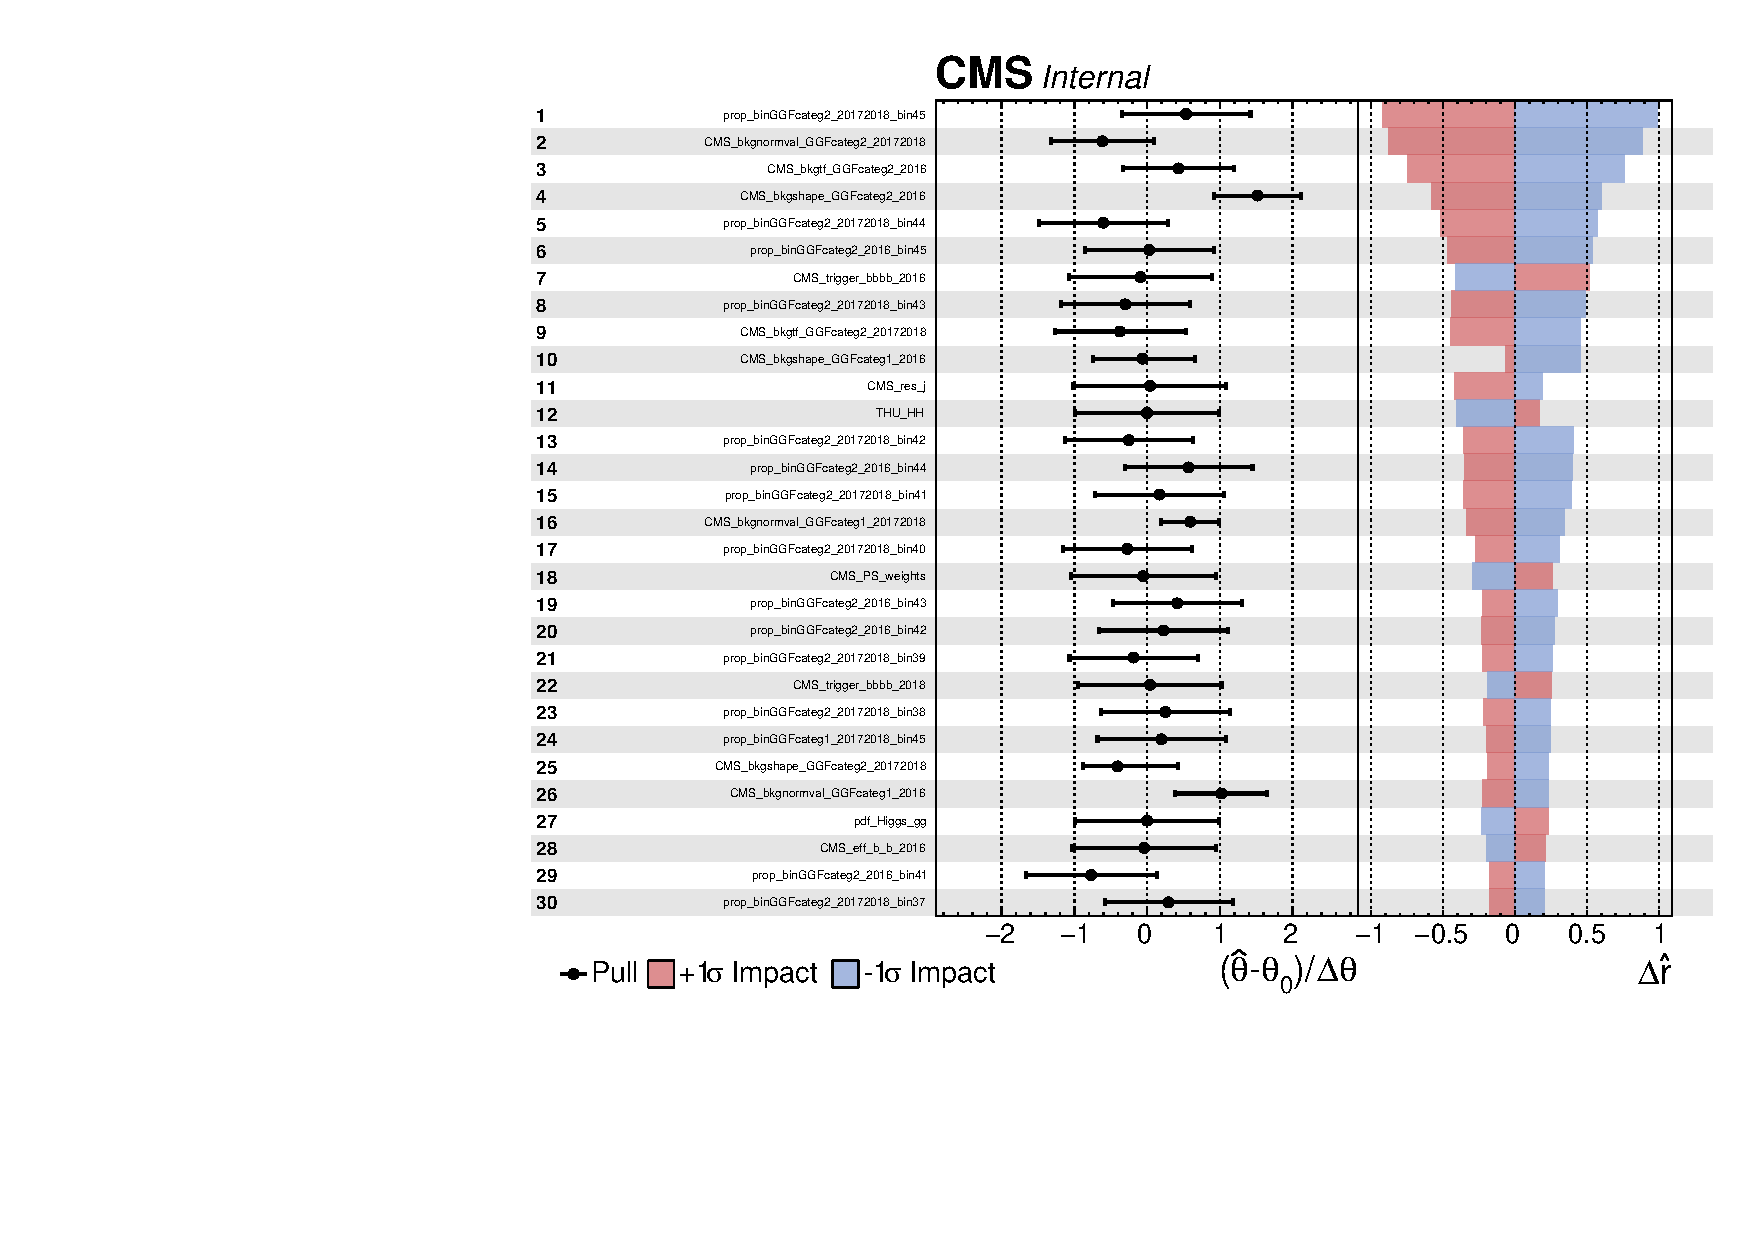
\includegraphics[width=0.85\textwidth,page=1]{Figures/Results/systematics/impacts_observed.pdf}
\caption[Observed impact of the highest systematic uncertainties on the measurement of the signal strength]{Observed impact of the highest systematic uncertainties on the measurement of the signal strength ($\hat{r}$) using all analysis categories.}
\label{fig:syst:observedimpacts}
\end{figure}

To quantify how compatible the background model is to the observed data, a goodness of fit test based on the saturated model method~\cite{statsaturatedmodel} is evaluated individually in each category, and simultaneously in all Run-2 categories. This method similar to the $\chi^{2}$, but has the advantage to be evaluated for arbitrary binned channels and parameters. A test statistic is computed first in the observed data. Then, it is computed for 1000 generated toys with $\mu$ left floating such that the estimation is independent of the presence or absence of signal. The test statistic toys distribution is compared to the one in observed in data to compute the compatibility p-value, as illustrated in Figure~5.7. The resulting p-values are presented Table~\ref{tab:anacompatibilty}. They demonstrate the excellent performance of the background model in each individual category and in all categories.

\begin{table}[htbp!]
\caption[Data-background model compatibility p-value obtained from the goodness of fit test in the analysis region observables]{\label{tab:anacompatibilty} Data-background model compatibility p-value obtained from the goodness of fit test applied to the observables in the $\mathrm{A_{SR}}$(4b) region.}
\centering
\begin{tabularx}{\textwidth}{lllX}
    \hline
    Dataset          & Subcategory    & Observable           &  Goodness of fit test p-value\\    
    \hline
    2016      & ggF category 1 & BDT output  & 76\% \\
    2016      & ggF category 2 & BDT output  & 57\% \\
    2016      & VBF category 1 & $\hhm$               & 72\% \\
    2016      & VBF category 2 & Counting experiment  & 99\% \\
    2017-2018 & ggF category 1 & BDT output  & 23\% \\
    2017-2018 & ggF category 2 & BDT output  & 62\% \\
    2017-2018 & VBF category 1 & $\hhm$               & 45\% \\
    2017-2018 & VBF category 2 & Counting experiment  & 41\% \\
    Run-2     & All            & All                  & 72\% \\ 
    \hline
\end{tabularx}
\end{table}

\subsection{Observed Distributions} \label{results:obsdistributions}
The distributions of the signal region observables in all categories (ggF cat.1, ggF cat.2, VBF cat.1 and VBF cat. 2) are presented in Figures~\ref{fig:bkgobservablesanatest2016} and~\ref{fig:bkgobservablesanatest20172018} for the 2016 and 2017-2018 datasets, respectively. The shown background model is the `post-fit' background and uncertainties obtained by maximum likelihood fit of the background-only model to the observed data. The background model describes well the data within the uncertainties in all categories. Figure~\ref{fig:log10sb} combines all distributions into a single one, made with bins of similar expected signal-to-background ratio, where SM ggF signal is assumed. No significant excess of data events is observed in the highest bins of the distribution by looking at the data/background ratio panel.  An underfluctuation of the data relative to the background model is observed in a few very sensitive bins, which correspond to the 2017-2018 ggF category 2. The underfluctuation in this category was studied in detail during the review, and it was concluded that it is of statistical nature. Therefore, the observed distributions are consistent with the background-only hypothesis.

\begin{figure}[htbp!]
\begin{center}
\captionsetup[subfigure]{justification=centering}
\subfloat[]{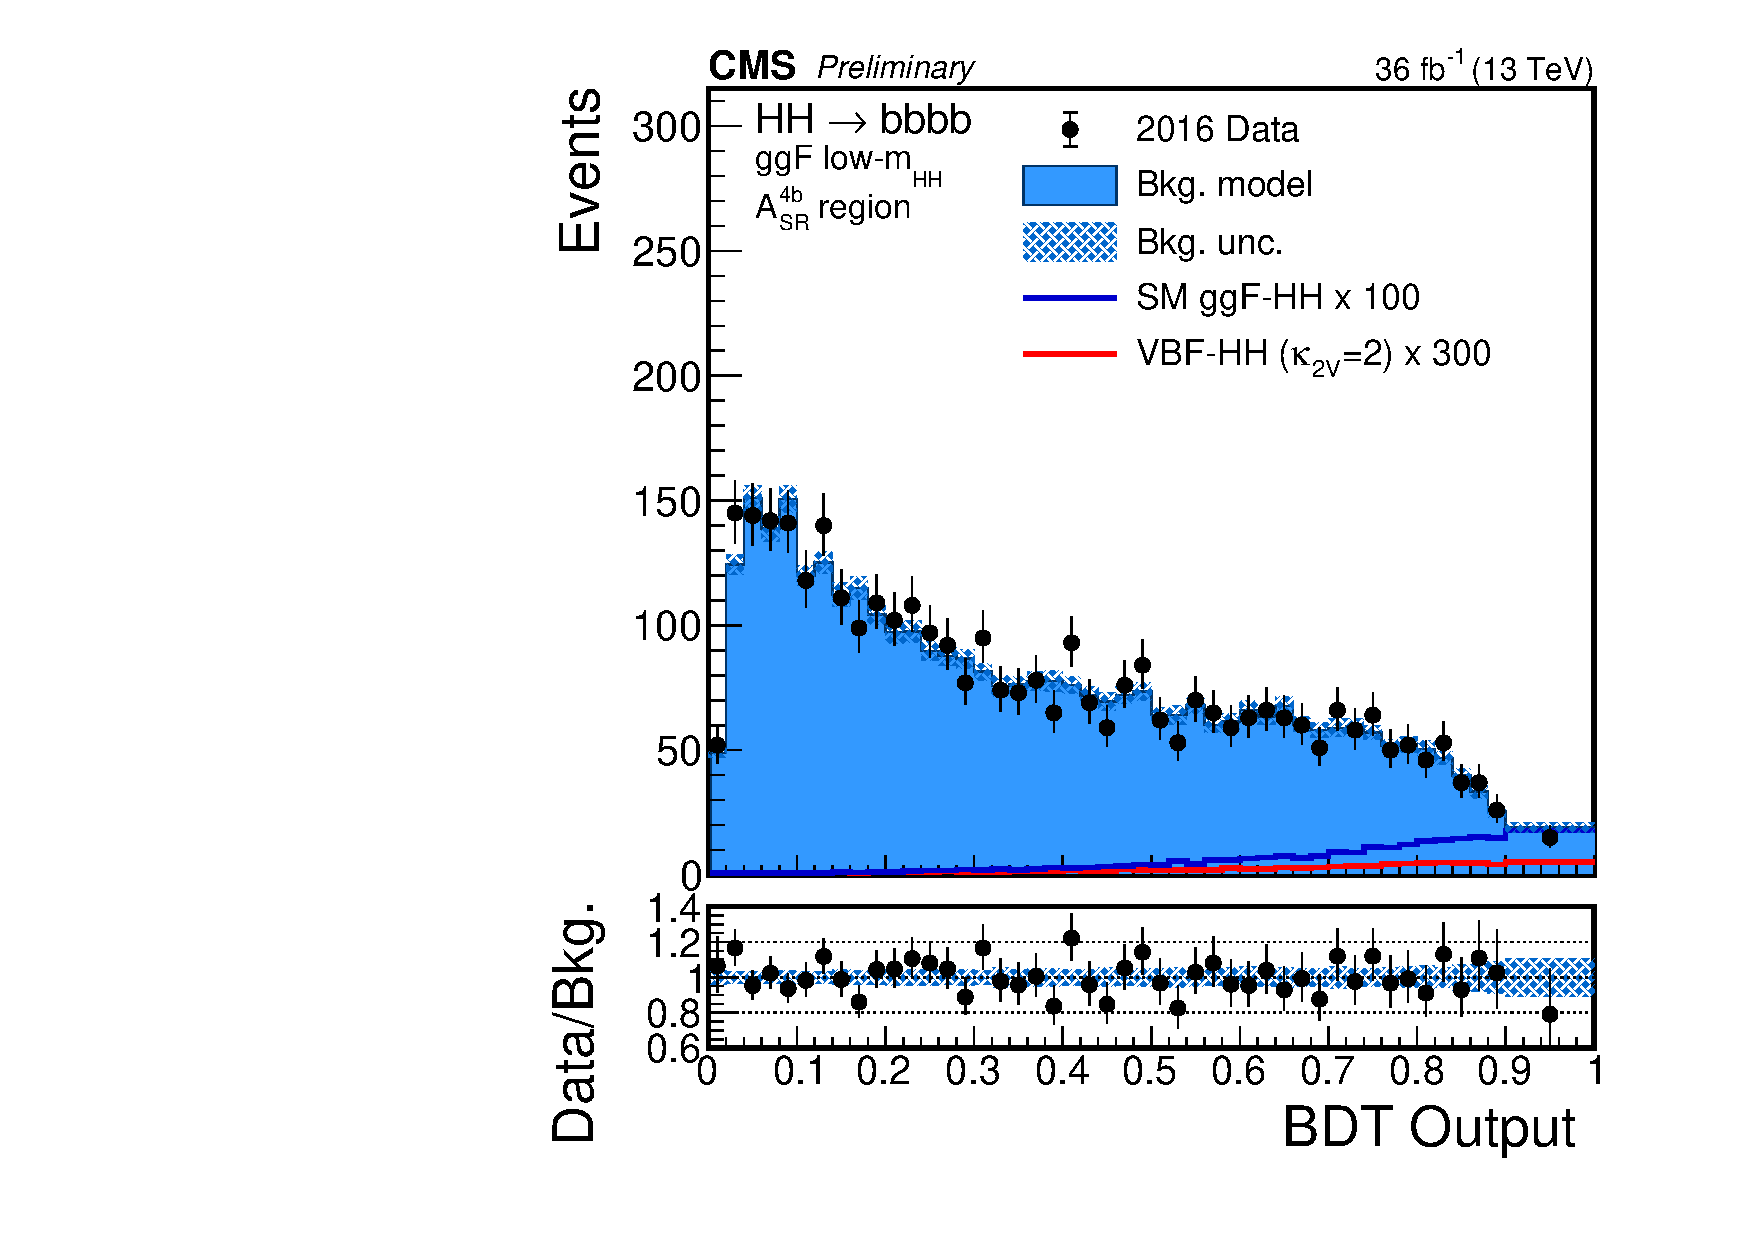
\includegraphics[width=0.50\linewidth]{Figures/Results/signalregion/2016/GGFcateg1_SR_110/plot2016_GGFMVA1_Btag4_GGFcateg1_SR_110_Histogram_postfit.pdf}}
\subfloat[]{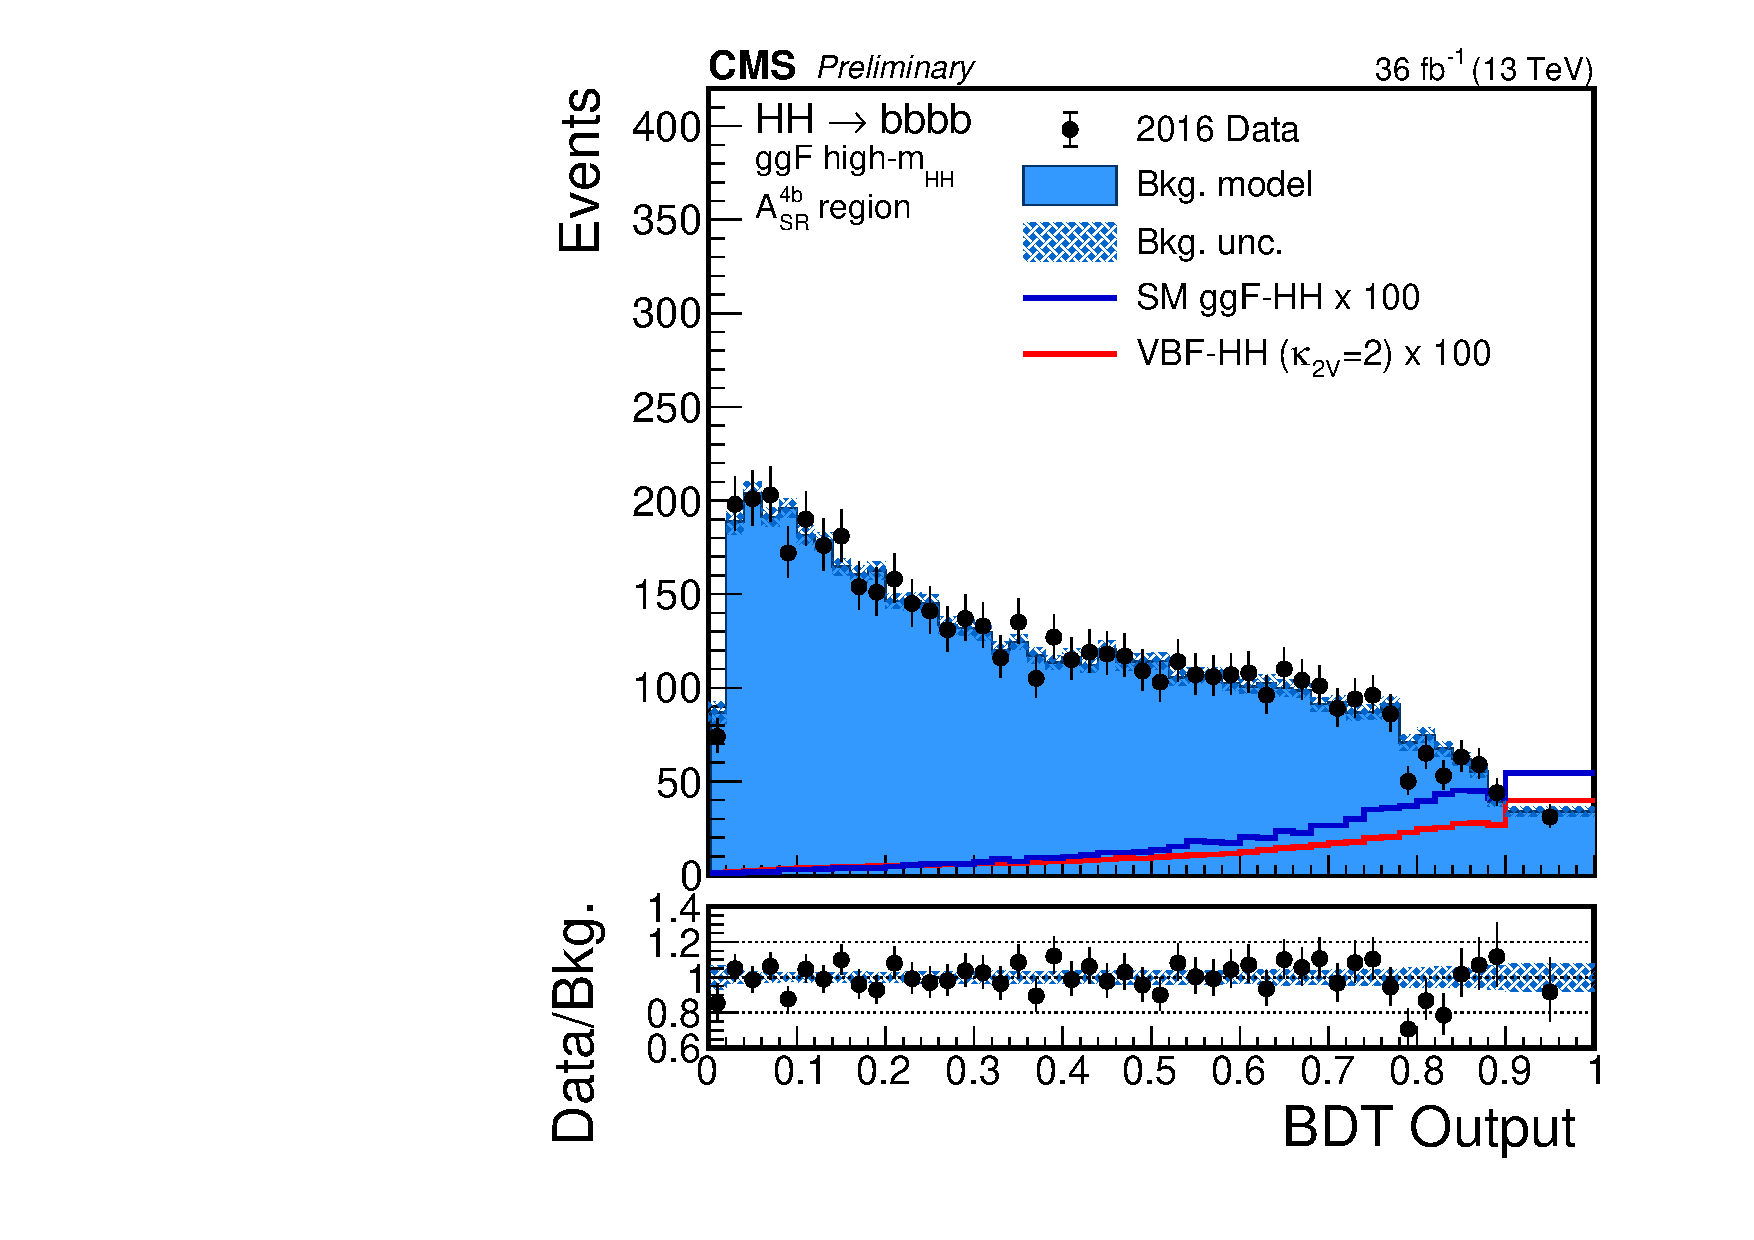
\includegraphics[width=0.50\linewidth]{Figures/Results/signalregion/2016/GGFcateg2_SR_110/plot2016_GGFMVA2_Btag4_GGFcateg2_SR_110_Histogram_postfit.pdf}}\\
\subfloat[]{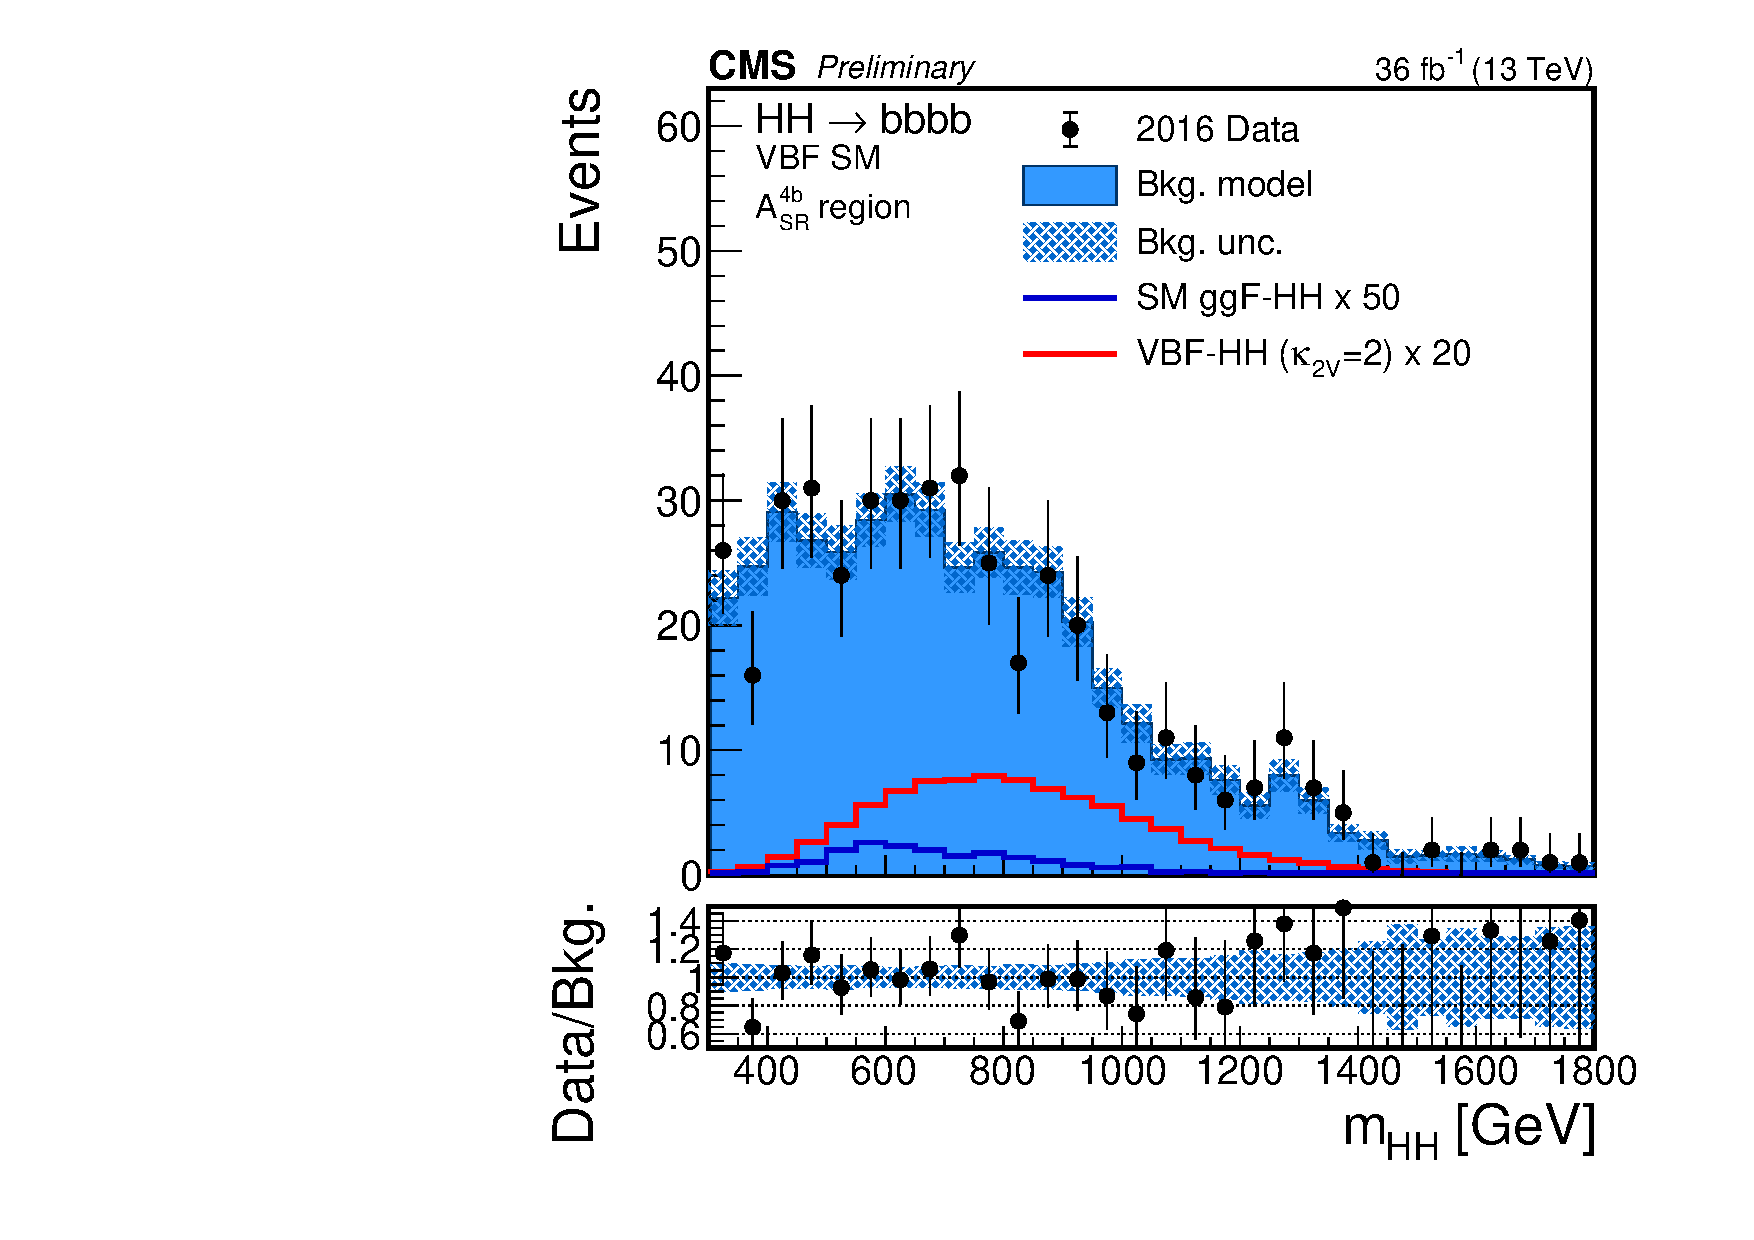
\includegraphics[width=0.50\linewidth]{Figures/Results/signalregion/2016/VBFcateg1_SR_110/plot2016_HH_m_1_Btag4_VBFcateg1_SR_110_Histogram_postfit.pdf}}
\subfloat[]{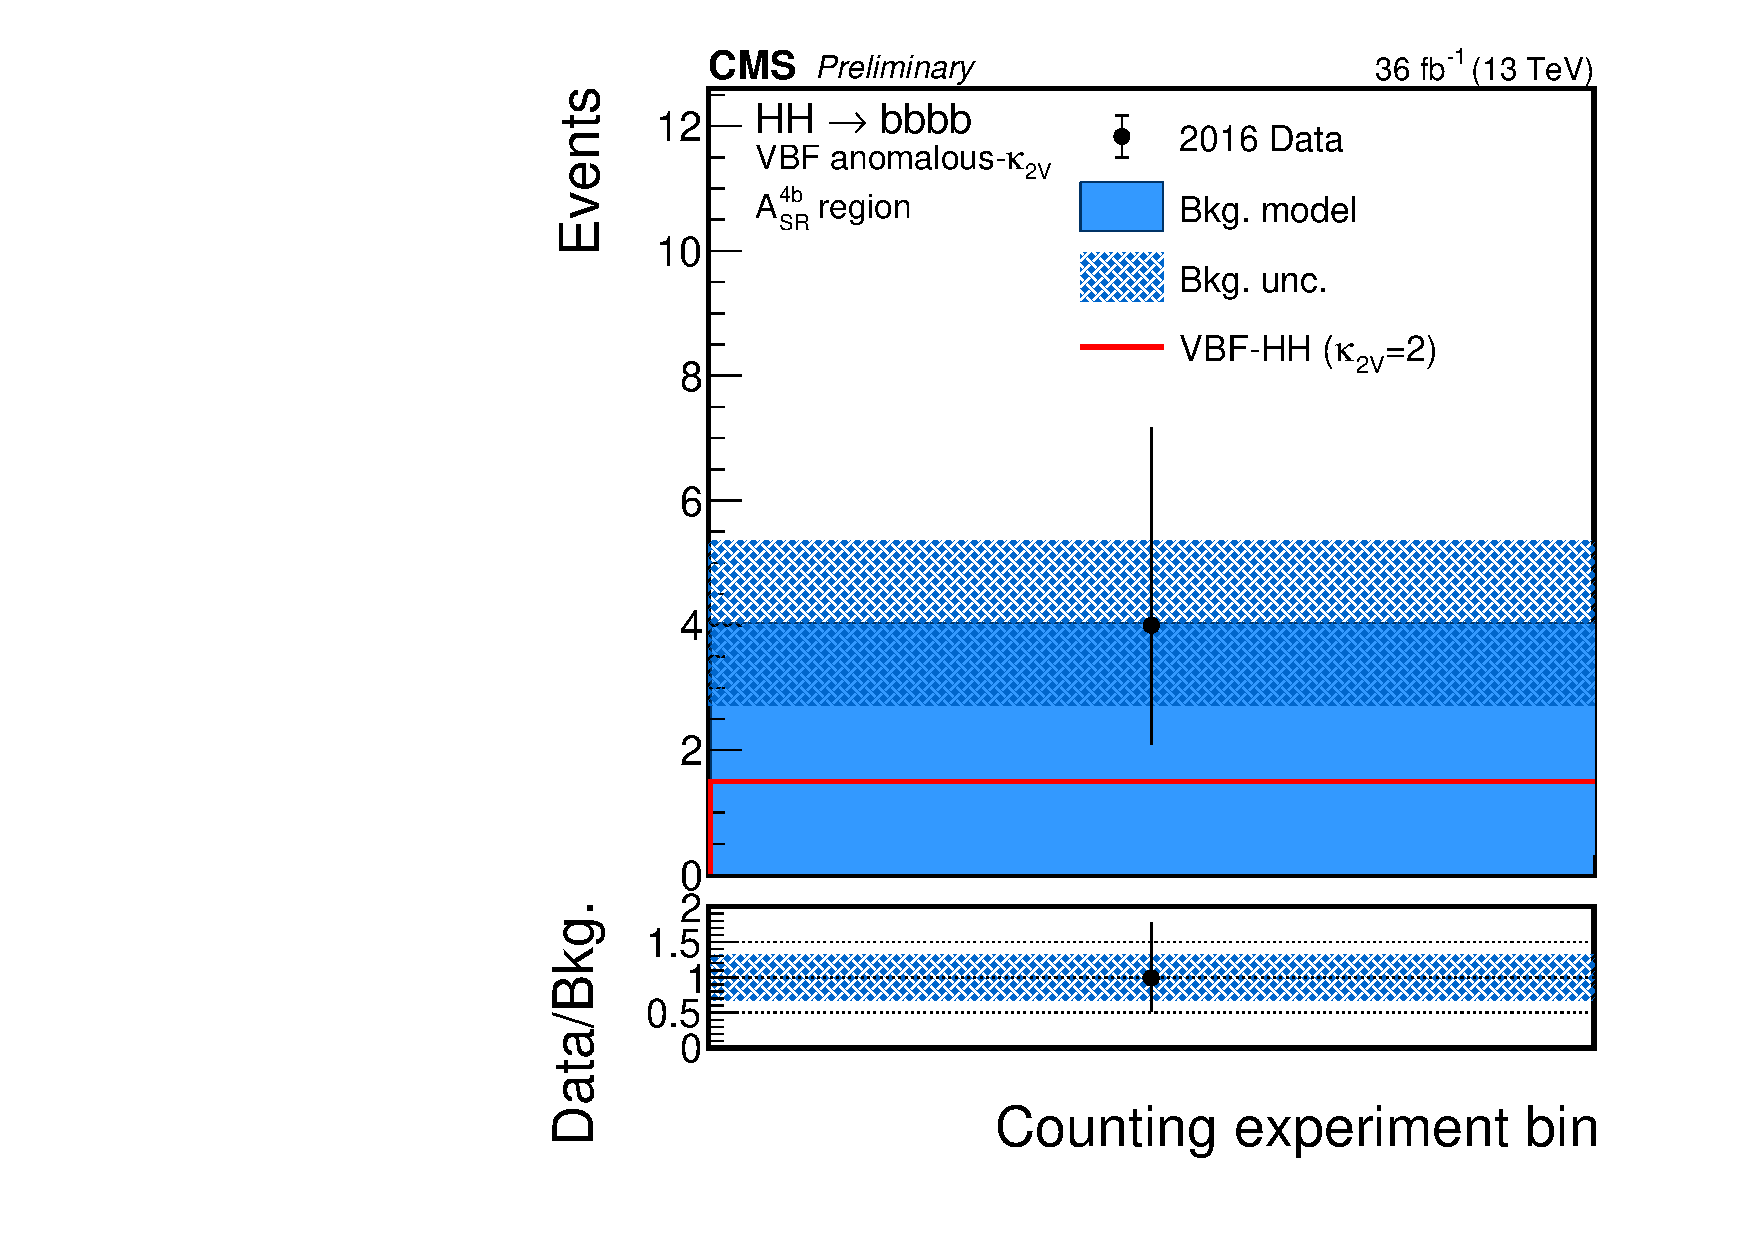
\includegraphics[width=0.50\linewidth]{Figures/Results/signalregion/2016/VBFcateg2_SR_110/plot2016_HH_m_2_Btag4_VBFcateg2_SR_110_Histogram_postfit.pdf}}
\end{center}
\caption[Observed distribution in the analysis signal regions for the 2016 data]{Observed distribution in the signal regions for 2016 data. A) ggF category 1, B) ggF category 2, C) VBF category 1, D) VBF Category 2. The presented background distributions are the one obtained after fitting the background prediction to the data floating the background uncertainties.}
\label{fig:bkgobservablesanatest2016}
\end{figure}

\begin{figure}[htbp!]
\begin{center}
\captionsetup[subfigure]{justification=centering}
\subfloat[]{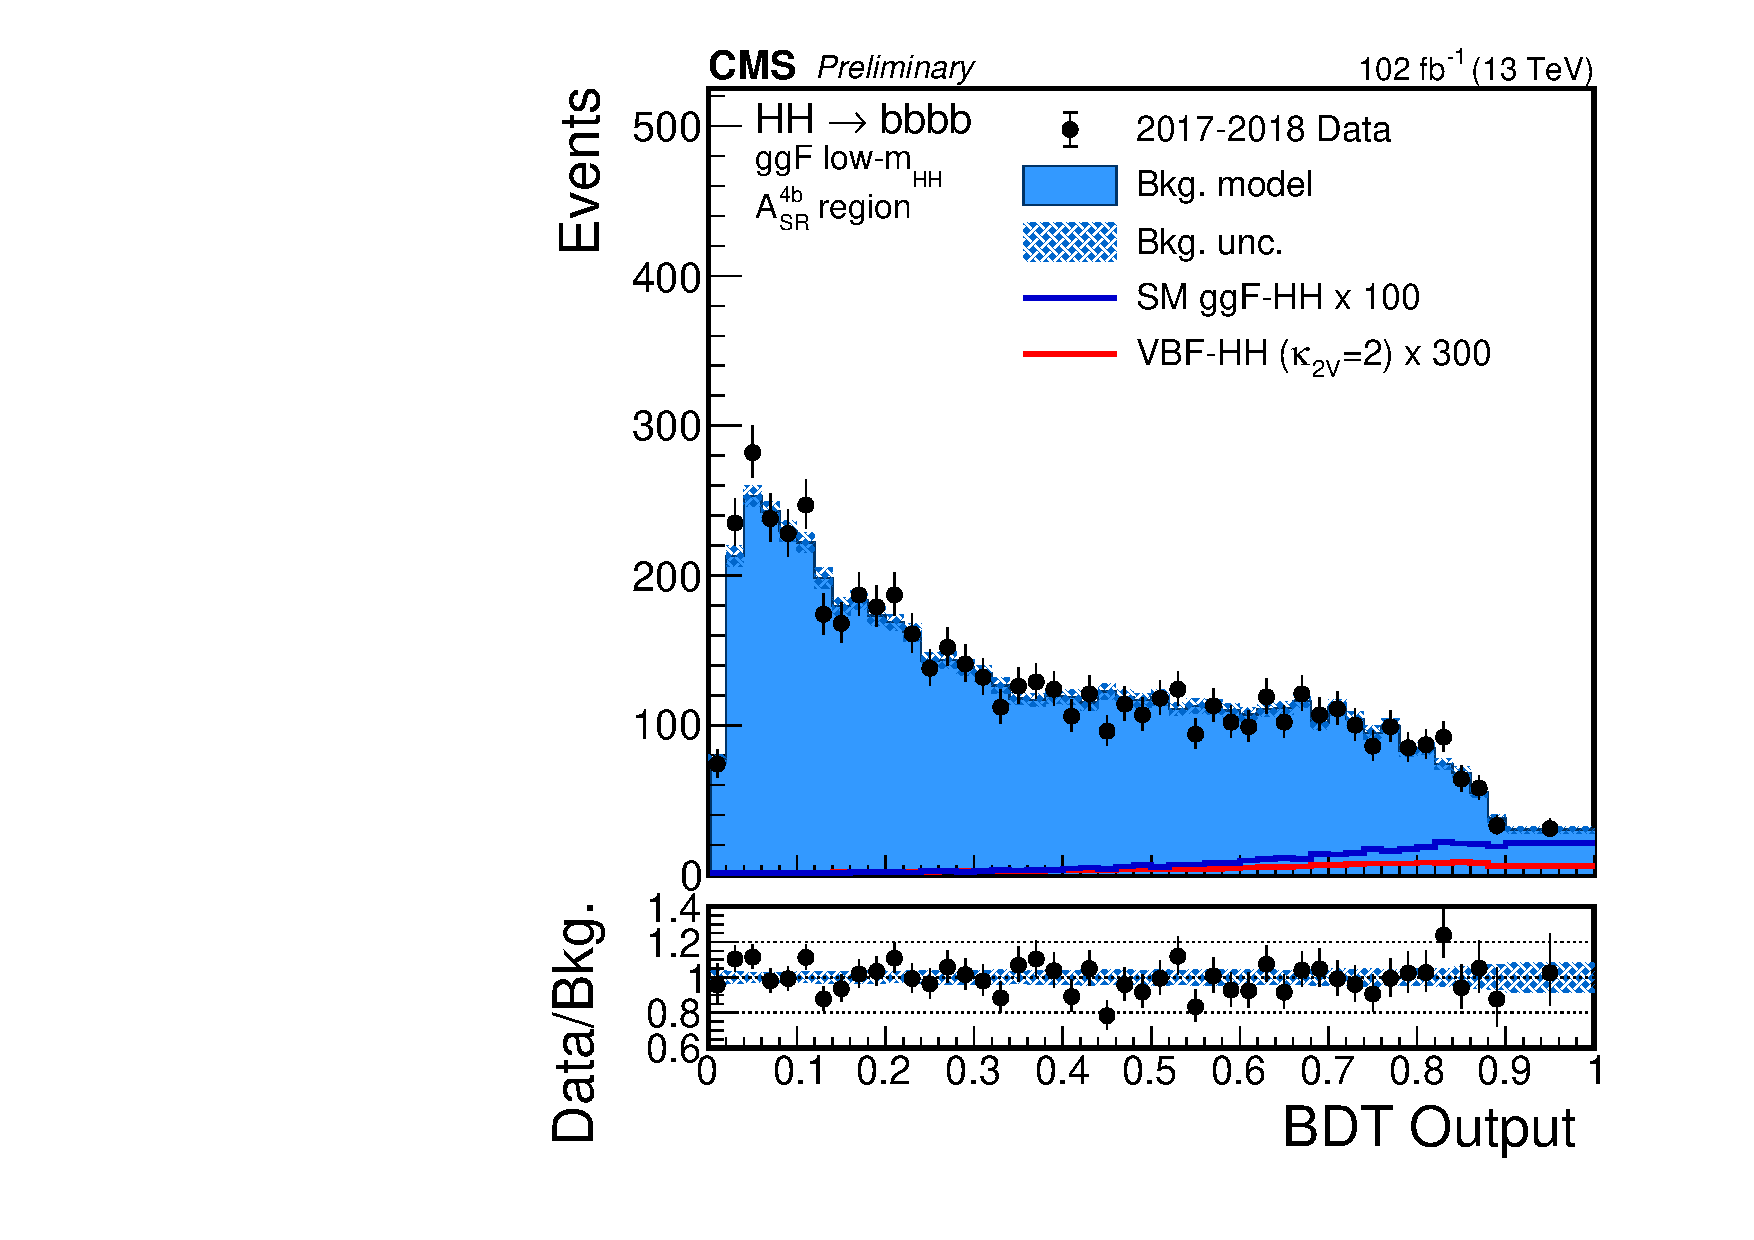
\includegraphics[width=0.50\linewidth]{Figures/Results/signalregion/20172018/GGFcateg1_SR_110/plot20172018_GGFMVA1_Btag4_GGFcateg1_SR_110_Histogram_postfit.pdf}}
\subfloat[]{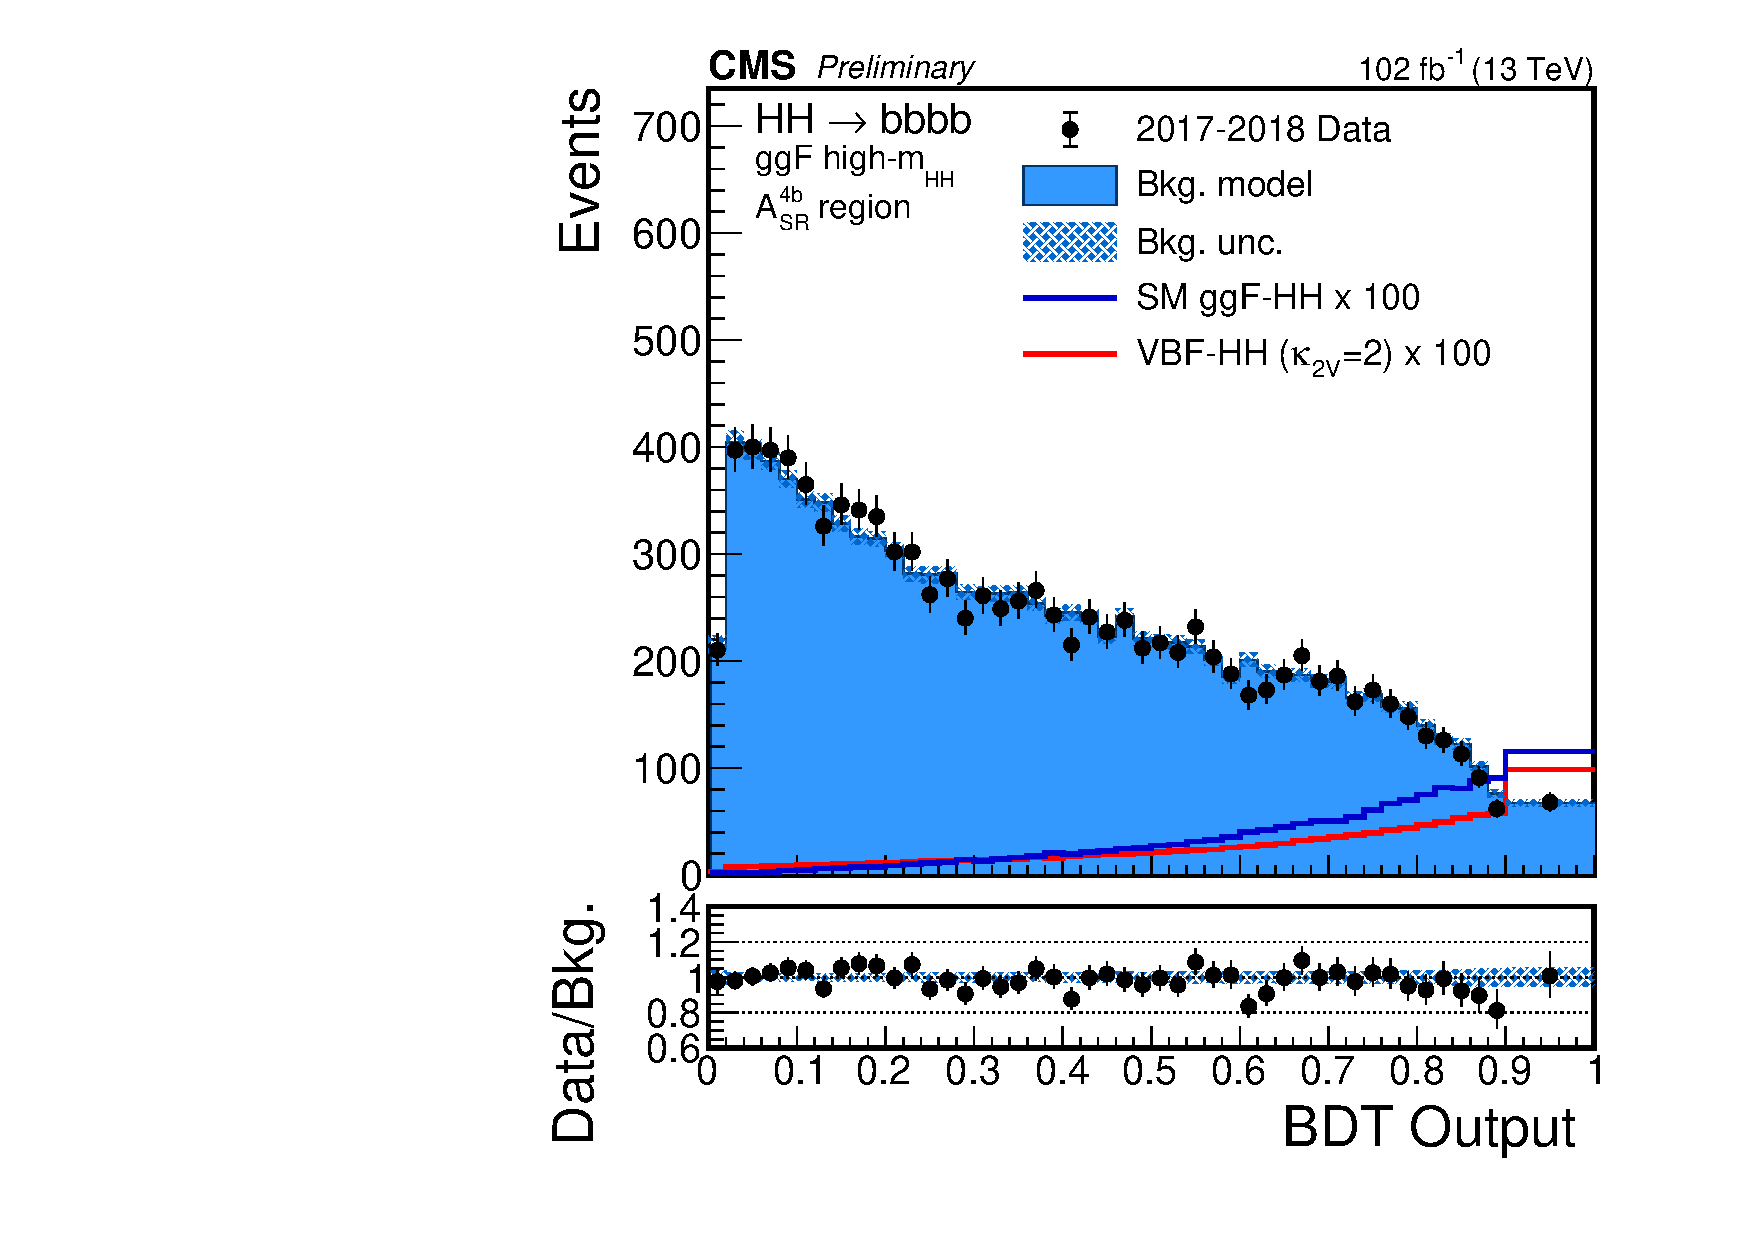
\includegraphics[width=0.50\linewidth]{Figures/Results/signalregion/20172018/GGFcateg2_SR_110/plot20172018_GGFMVA2_Btag4_GGFcateg2_SR_110_Histogram_postfit.pdf}}\\
\subfloat[]{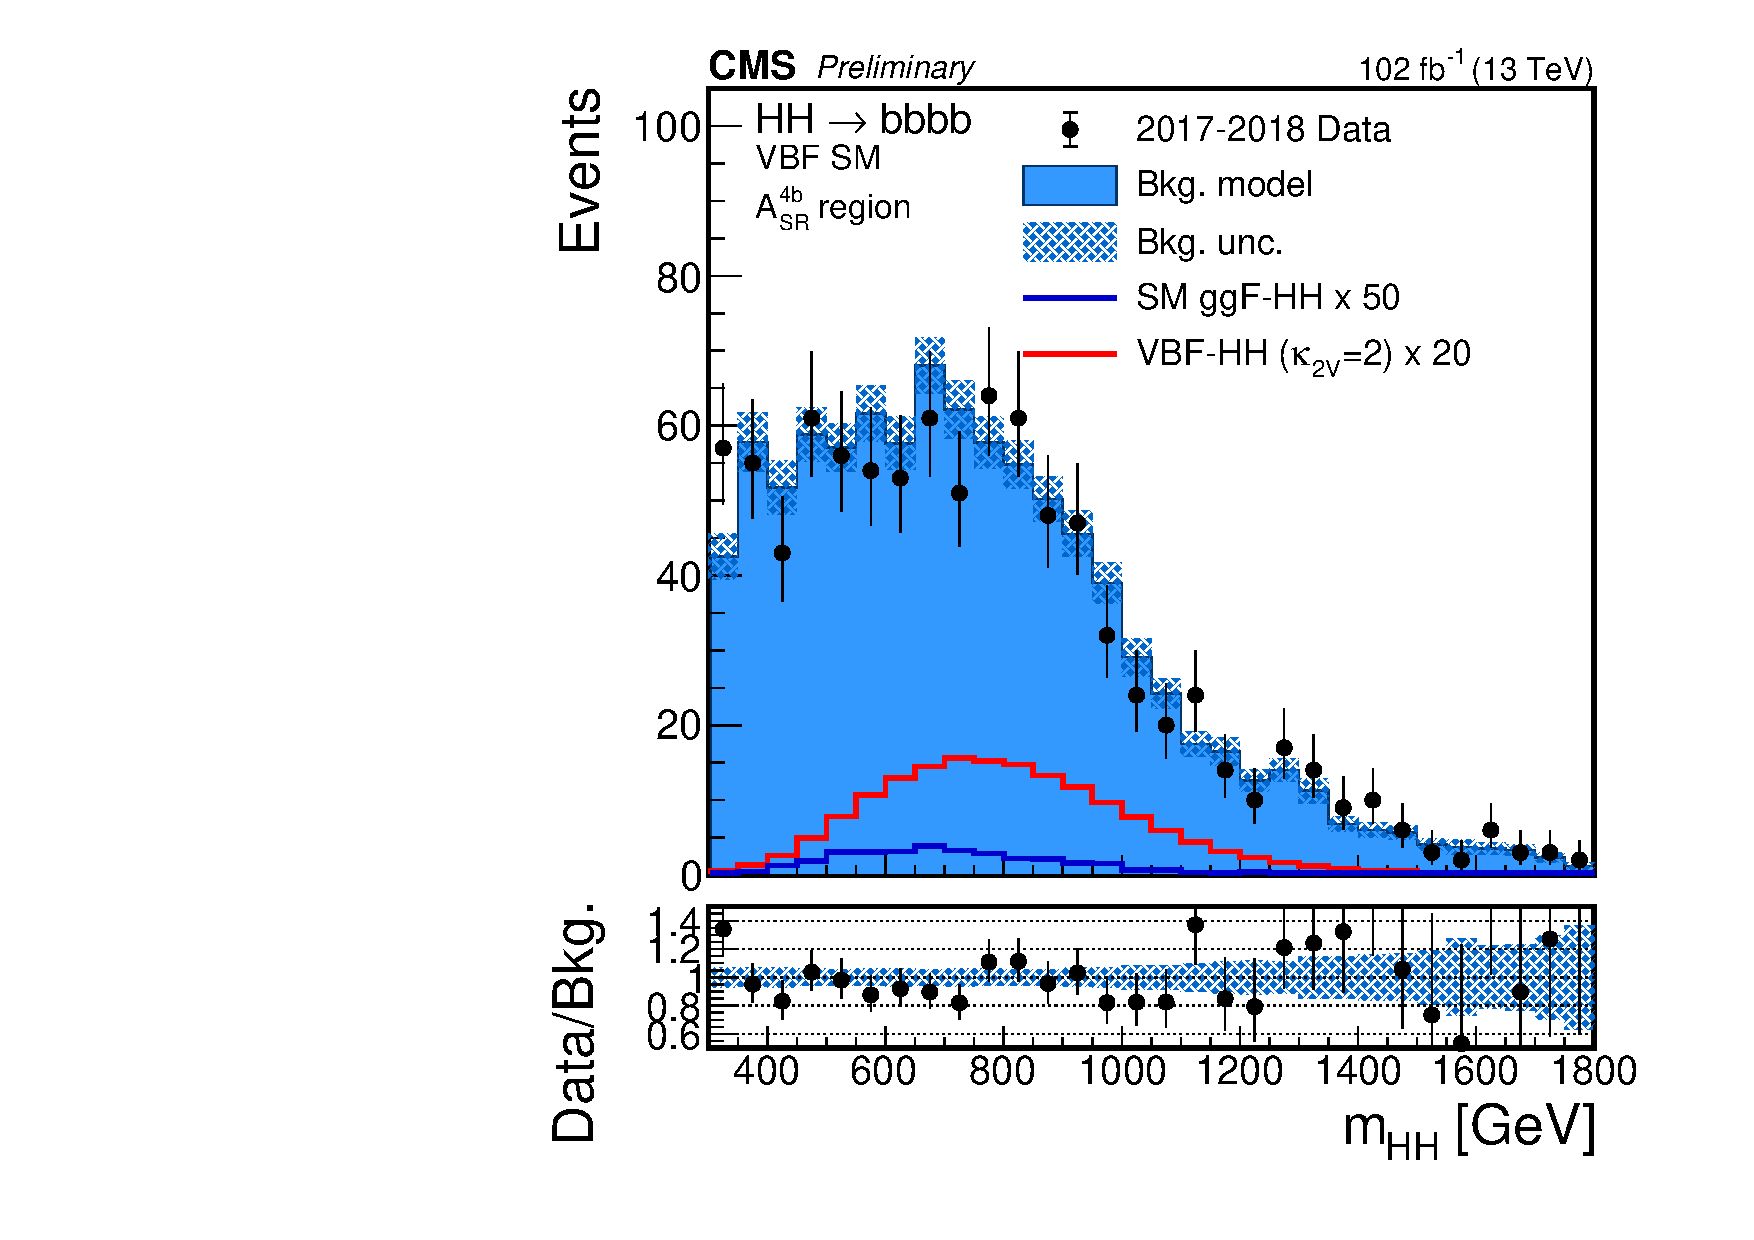
\includegraphics[width=0.50\linewidth]{Figures/Results/signalregion/20172018/VBFcateg1_SR_110/plot20172018_HH_m_1_Btag4_VBFcateg1_SR_110_Histogram_postfit.pdf}}
\subfloat[]{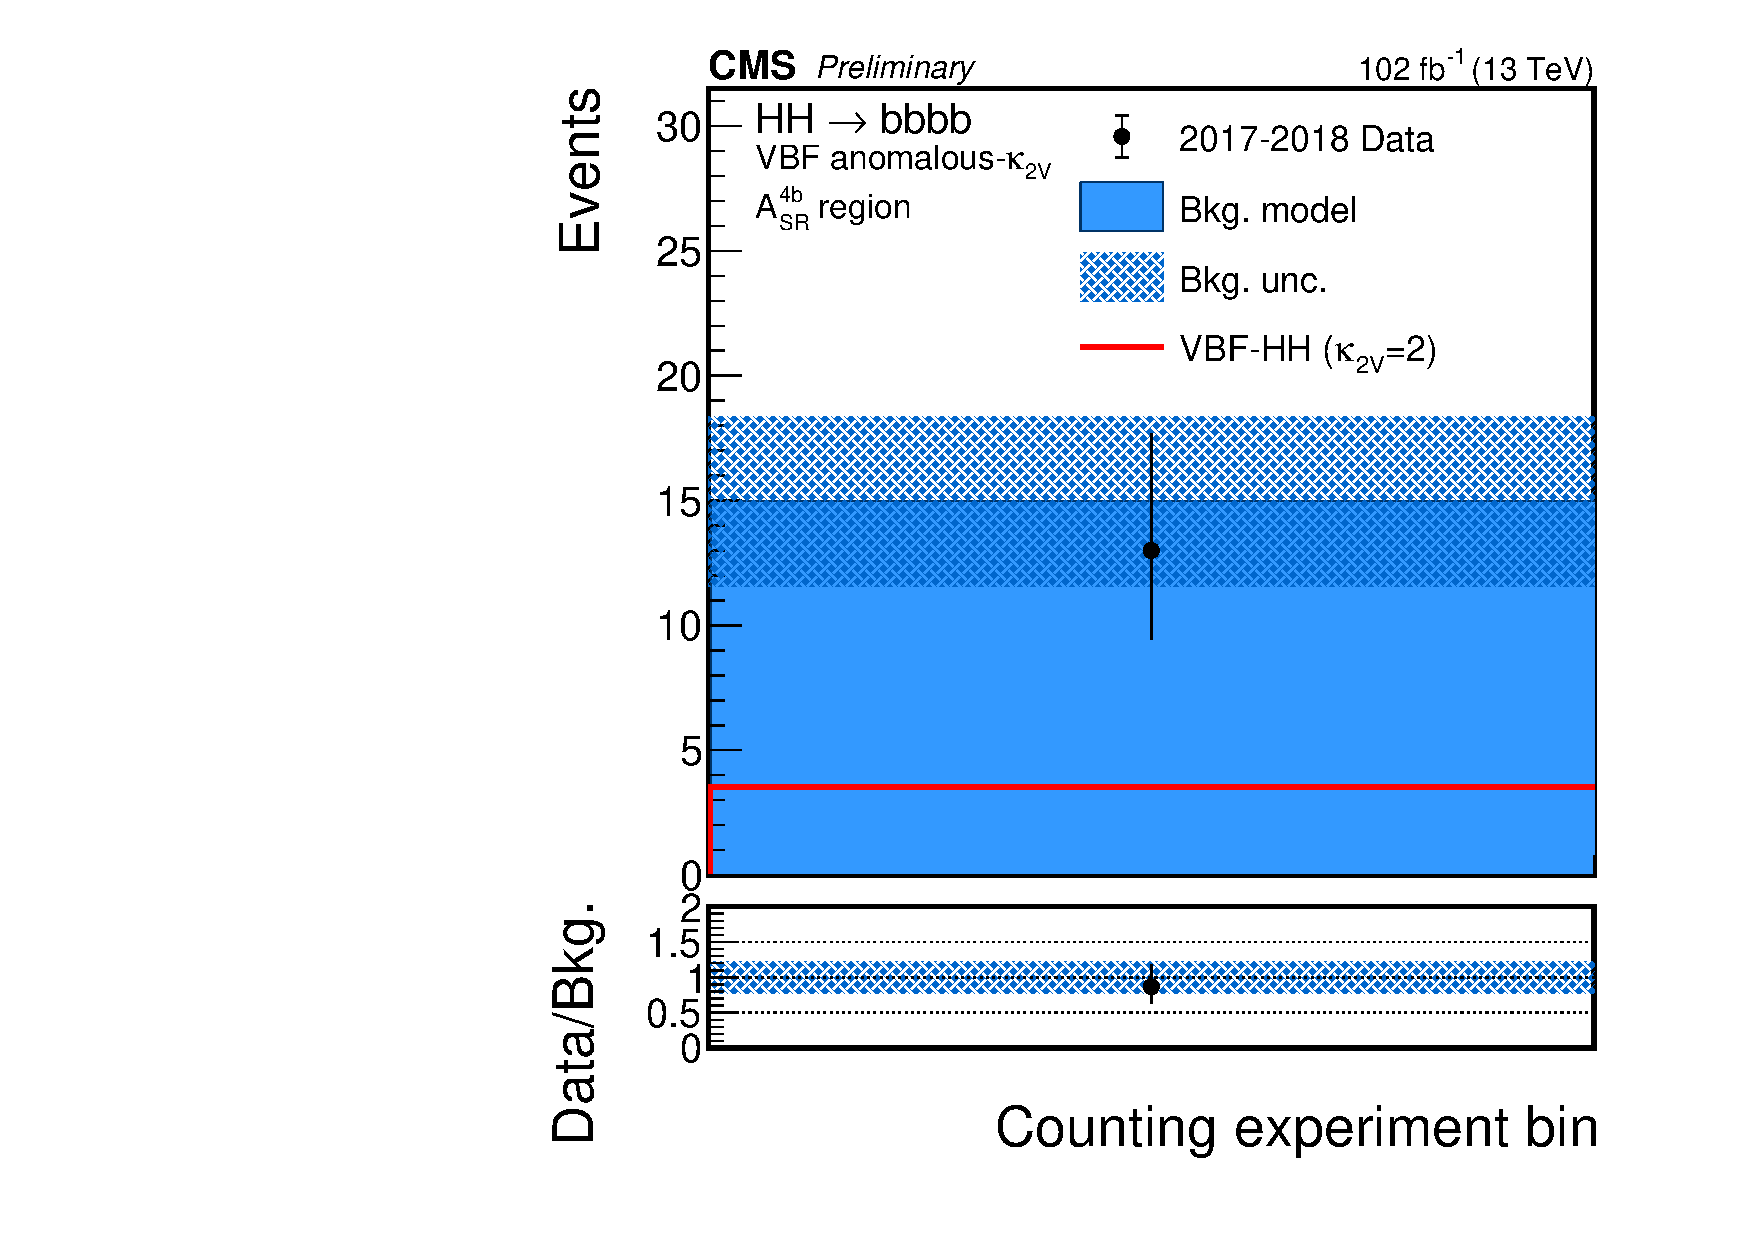
\includegraphics[width=0.50\linewidth]{Figures/Results/signalregion/20172018/VBFcateg2_SR_110/plot20172018_HH_m_2_Btag4_VBFcateg2_SR_110_Histogram_postfit.pdf}}
\end{center}
\caption[Distributions of the observables in the analysis signal regions for the 2017-2018 data]{Distributions of the observables in the signal regions for 2017-2018 data. A) ggF category 1, B) ggF category 2, C) VBF category 1, D) VBF Category 2. The presented background distributions are the one obtained after fitting the background prediction to the data floating the background uncertainties.}
\label{fig:bkgobservablesanatest20172018}
\end{figure}

\clearpage
\begin{figure*}[ht!]
\centering
{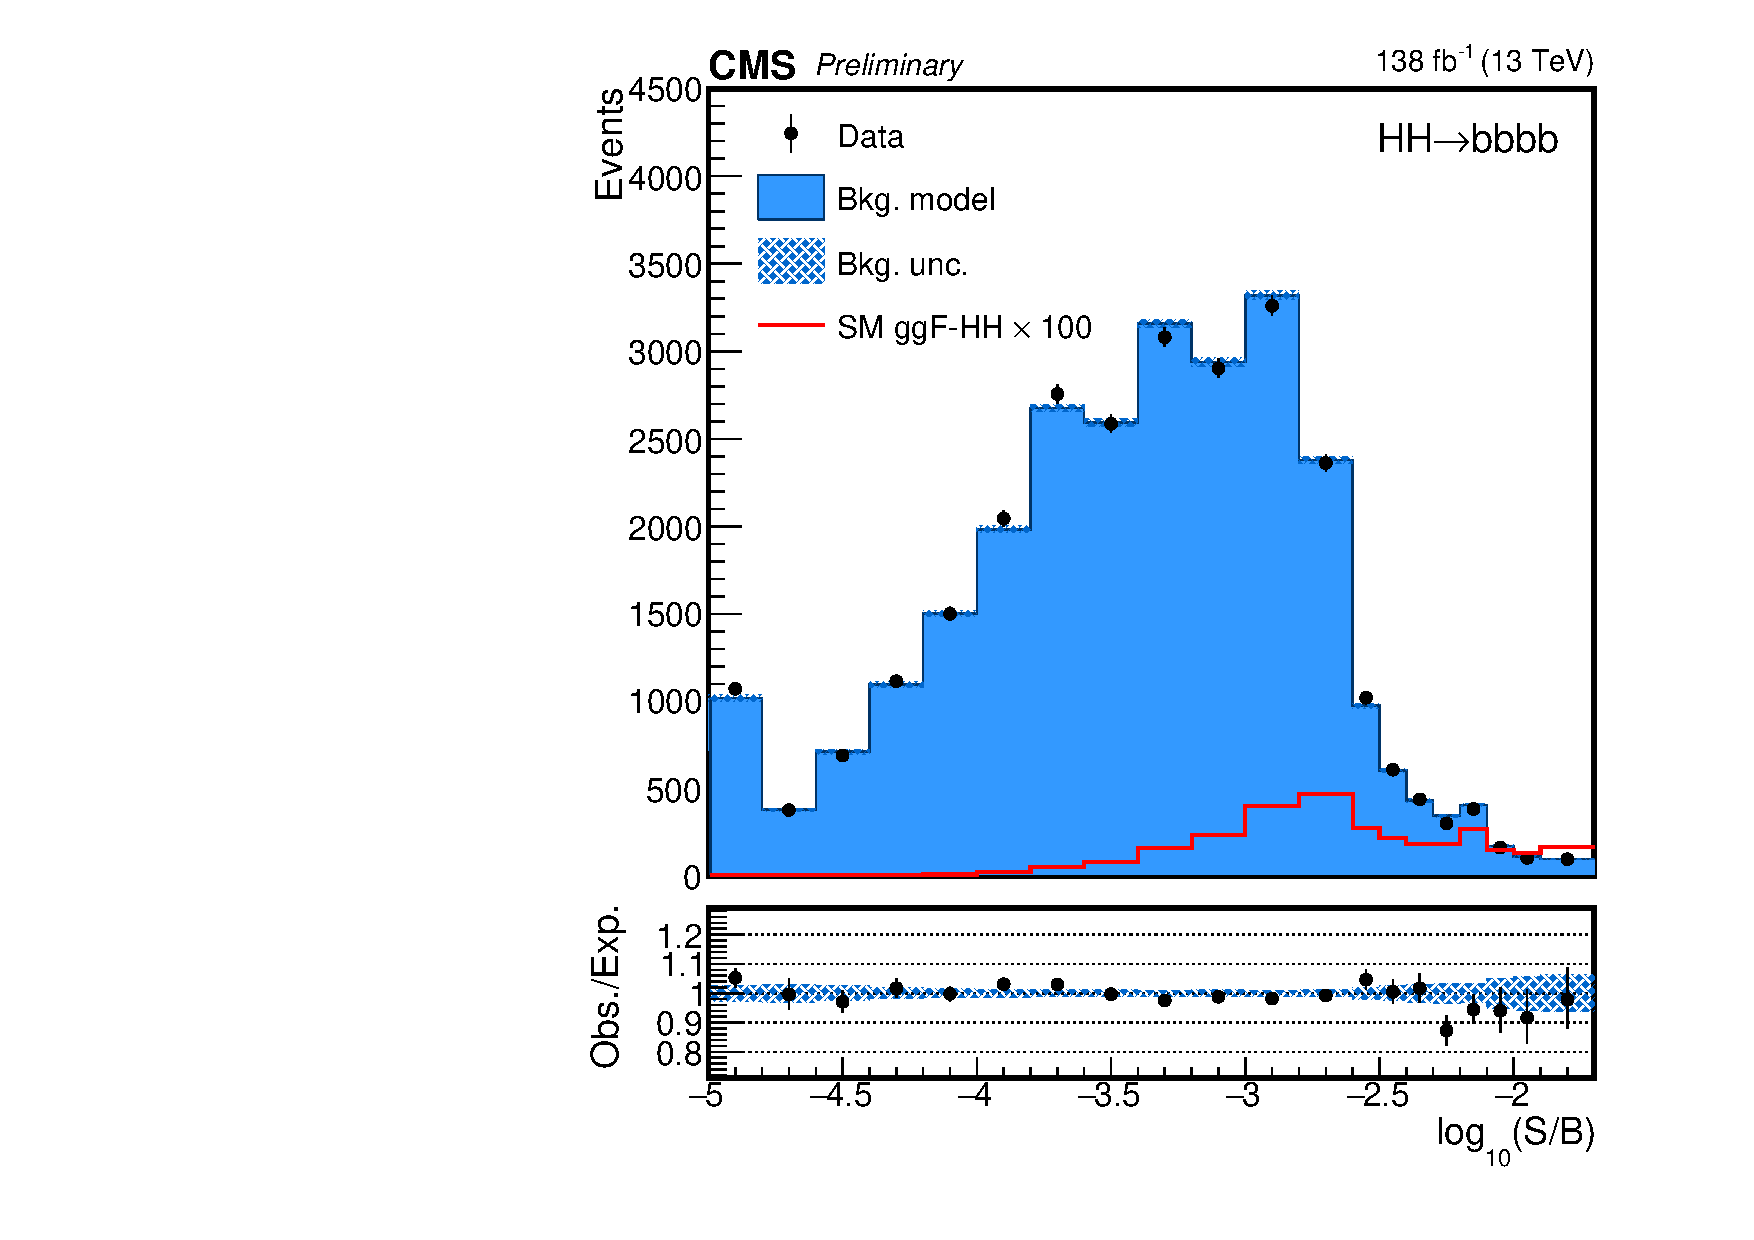
\includegraphics[width=0.5\linewidth]{Figures/Results/additional/CMS-PAS-HIG-20-005_Figure-aux_014.pdf}}
\caption[Distribution of the expected signal-to-background ratio for events selected in all categories and datasets]{\label{fig:log10sb}
Distribution of the expected signal-to-background ratio for events selected in all categories and datasets.}
\end{figure*}

\section{Upper Limits} \label{results:limits}
Under the hypothesis of absence of signal in the observed data with respect to the background, one can set  95 \% CL upper limits on the signal strength parameter $\mu$, which is then translated into a limit on the HH production cross section. The limits are computed using the asymptotic CLs method using the statistical model described in Subsection~\ref{results:statmodel}. The final results are obtained combining the limits from all categories and years. In the figures below, green and yellow bands indicate the regions containing 68 and 95\% of the distribution of limits expected under the background-only hypothesis, respectively.

The observed (expected) upper limits on the SM signal strength parameter ($\mathrm{\mu=\sigma_{HH}/\sigma_{HH}^{SM}}$) is set 3.7 (7.3). The breakdown of the contributions to this constraint by year and category are presented in Figure~\ref{fig:limitsbyyear} and Figure~\ref{fig:limitsbycateg}, respectively. The results show that the largest observed and expected constraint is obtained in the 2017-2018 ggF category 2.

\begin{figure*}[!htb]
\centering
{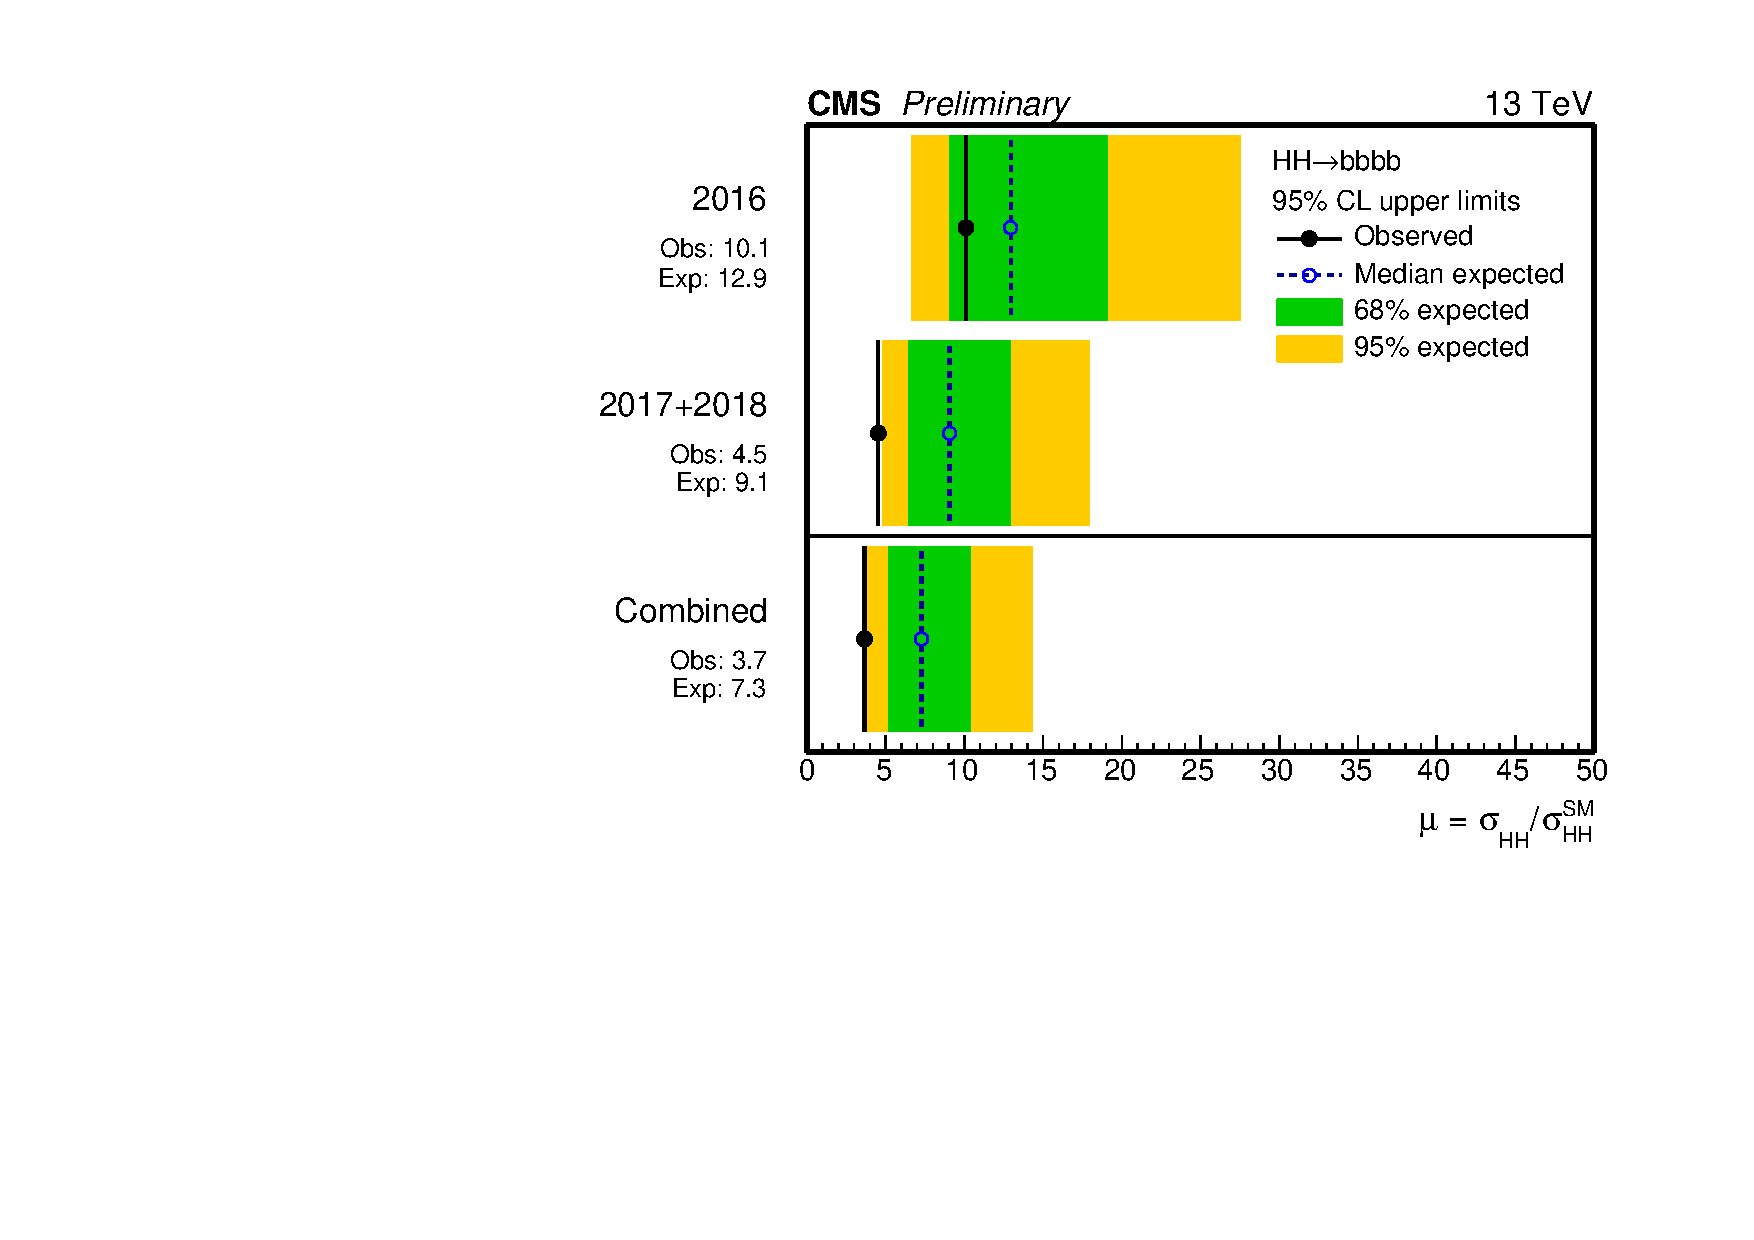
\includegraphics[width=0.55\linewidth] {Figures/Results/additional/CMS-PAS-HIG-20-005_Figure-aux_011.pdf}}
\caption[Observed and expected 95\% CL limits on the standard model Higgs boson pair (HH) production signal strength breakdown by year]{\label{fig:limitsbyyear}
Observed and expected 95\% CL limits on the standard model Higgs boson pair (HH) production signal strength ($\mu$) breakdown by year.}
\end{figure*}

\begin{figure*}[!htb]
\centering
{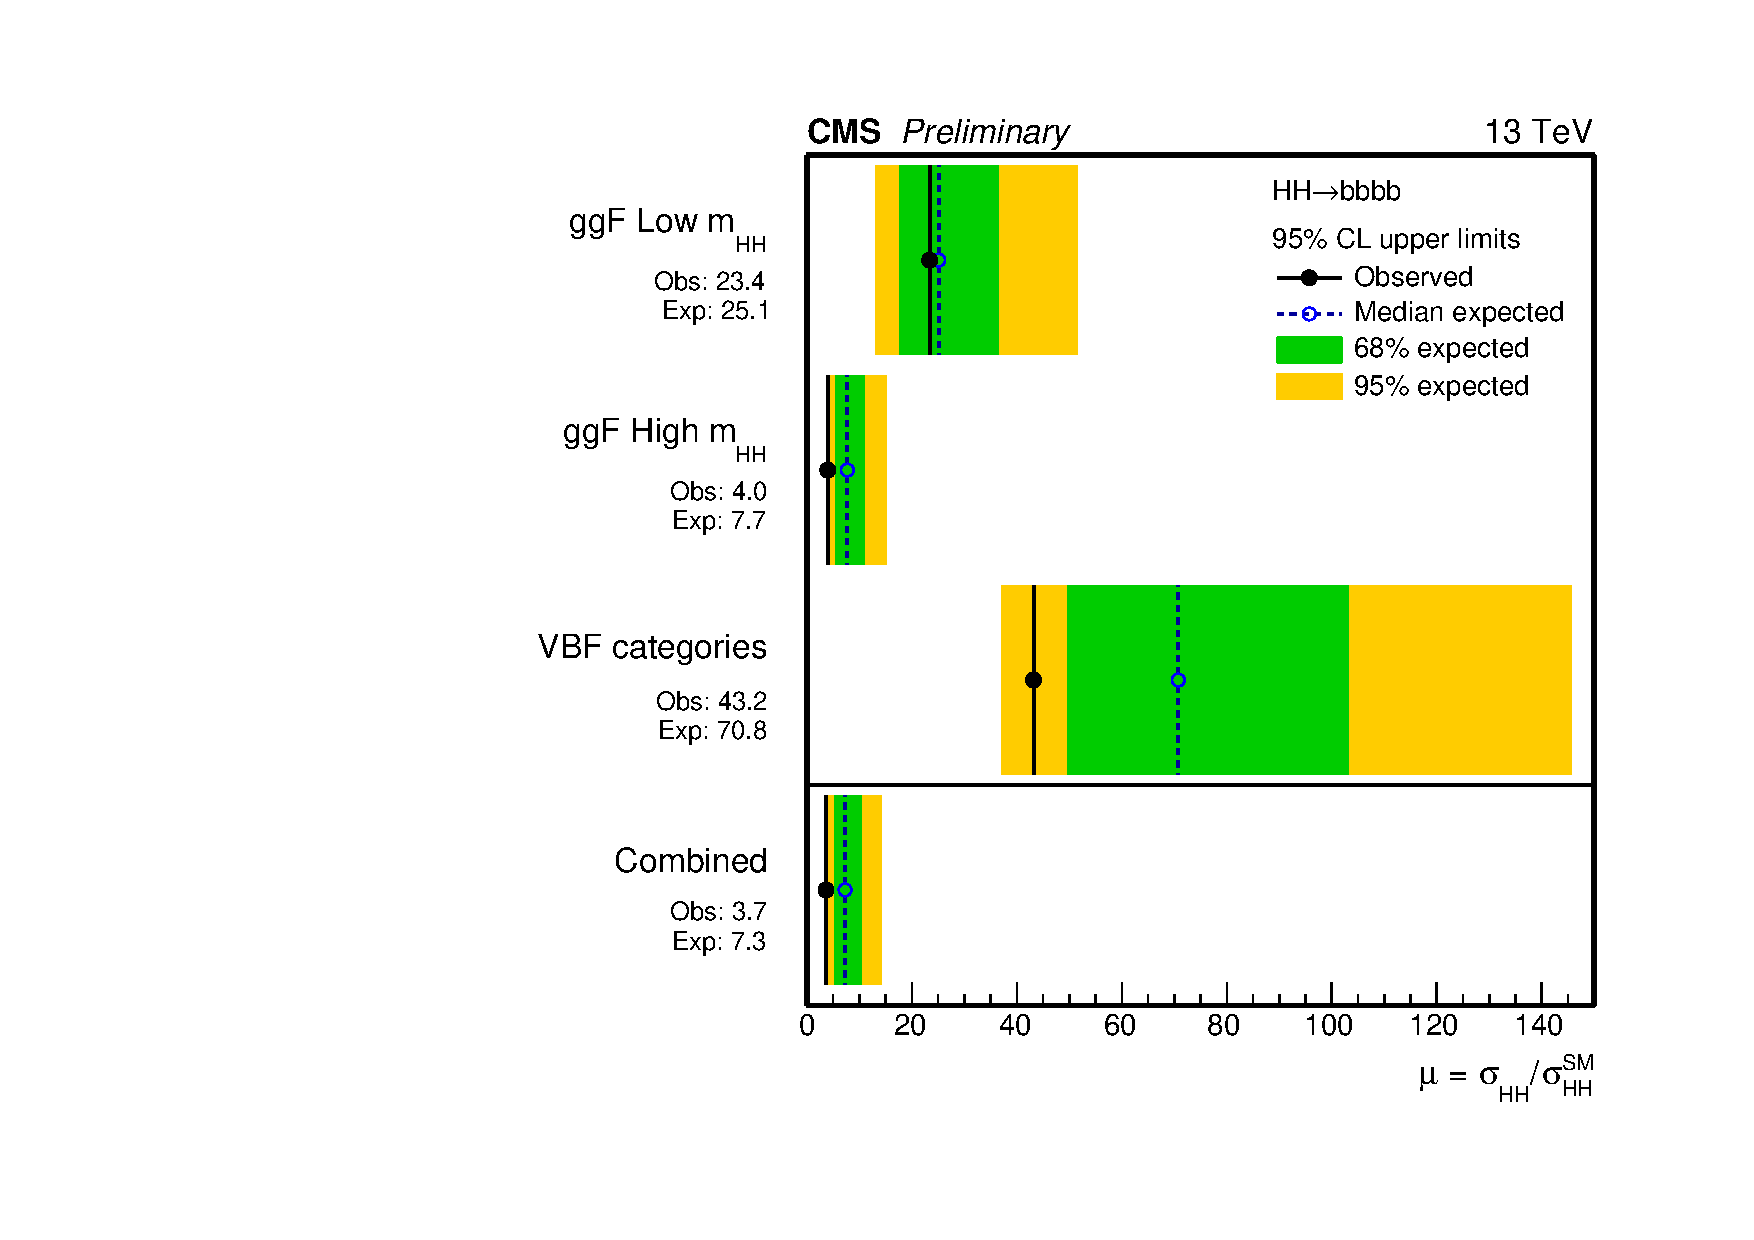
\includegraphics[width=0.5\linewidth] {Figures/Results/additional/CMS-PAS-HIG-20-005_Figure-aux_012.pdf}}
\caption[Observed and expected 95\% CL limits on the standard model Higgs boson pair (HH) production signal strength breakdown by category]{\label{fig:limitsbycateg}
Observed and expected 95\% CL limits on the standard model Higgs boson pair (HH) production signal strength ($\mu$) breakdown by category.}
\end{figure*}

The results are also interpreted as a limit on the SM cross section ($\mathrm{\sigma_{SM}^{HH}}$). The observed (expected) upper limit on the HH production cross section is set at 118 (239) fb. At the time of writing this dissertation, this is the stringent constraint on this process at the LHC. In addition, the observed (expected) limit on the VBF production cross section is set at 390 (711) fb, where the SM ggF signal is fixed as background.

Cross section limits are also obtained in the context of the anomalous SM couplings and non-SM couplings. Couplings that are not indicated on the horizontal axis are set to the SM prediction. Upper limits on the HH production cross section are derived as a function of the $\kl$ coupling modifier as illustrated in Figure~\ref{fig:ULscans} A). These limits are compared to the theoretical cross section (pink line) to obtain the observed (expected) allowed interval of $-2.3<\kl<9.4$ ($-5.0<\kl<12.0$) at 95\% CL. Moreover, upper limits on the VBF HH production cross section are also set as a function of the $\kvv$ coupling modifier, presented in Figure~\ref{fig:ULscans} B). The observed (expected) allowed interval of $-0.1<\kvv<2.2$ ($-0.4<\kvv<2.5$) at 95\% CL. In addition, Figure~\ref{fig:benchmarks} shows the observed (expected) upper limits are also set on the production cross section of the twelve EFT benchmarks presented section~\ref{hh:BSMcouplings} 

\begin{figure*}[!htb]
\captionsetup[subfigure]{justification=centering}
\centering
\subfloat[]{{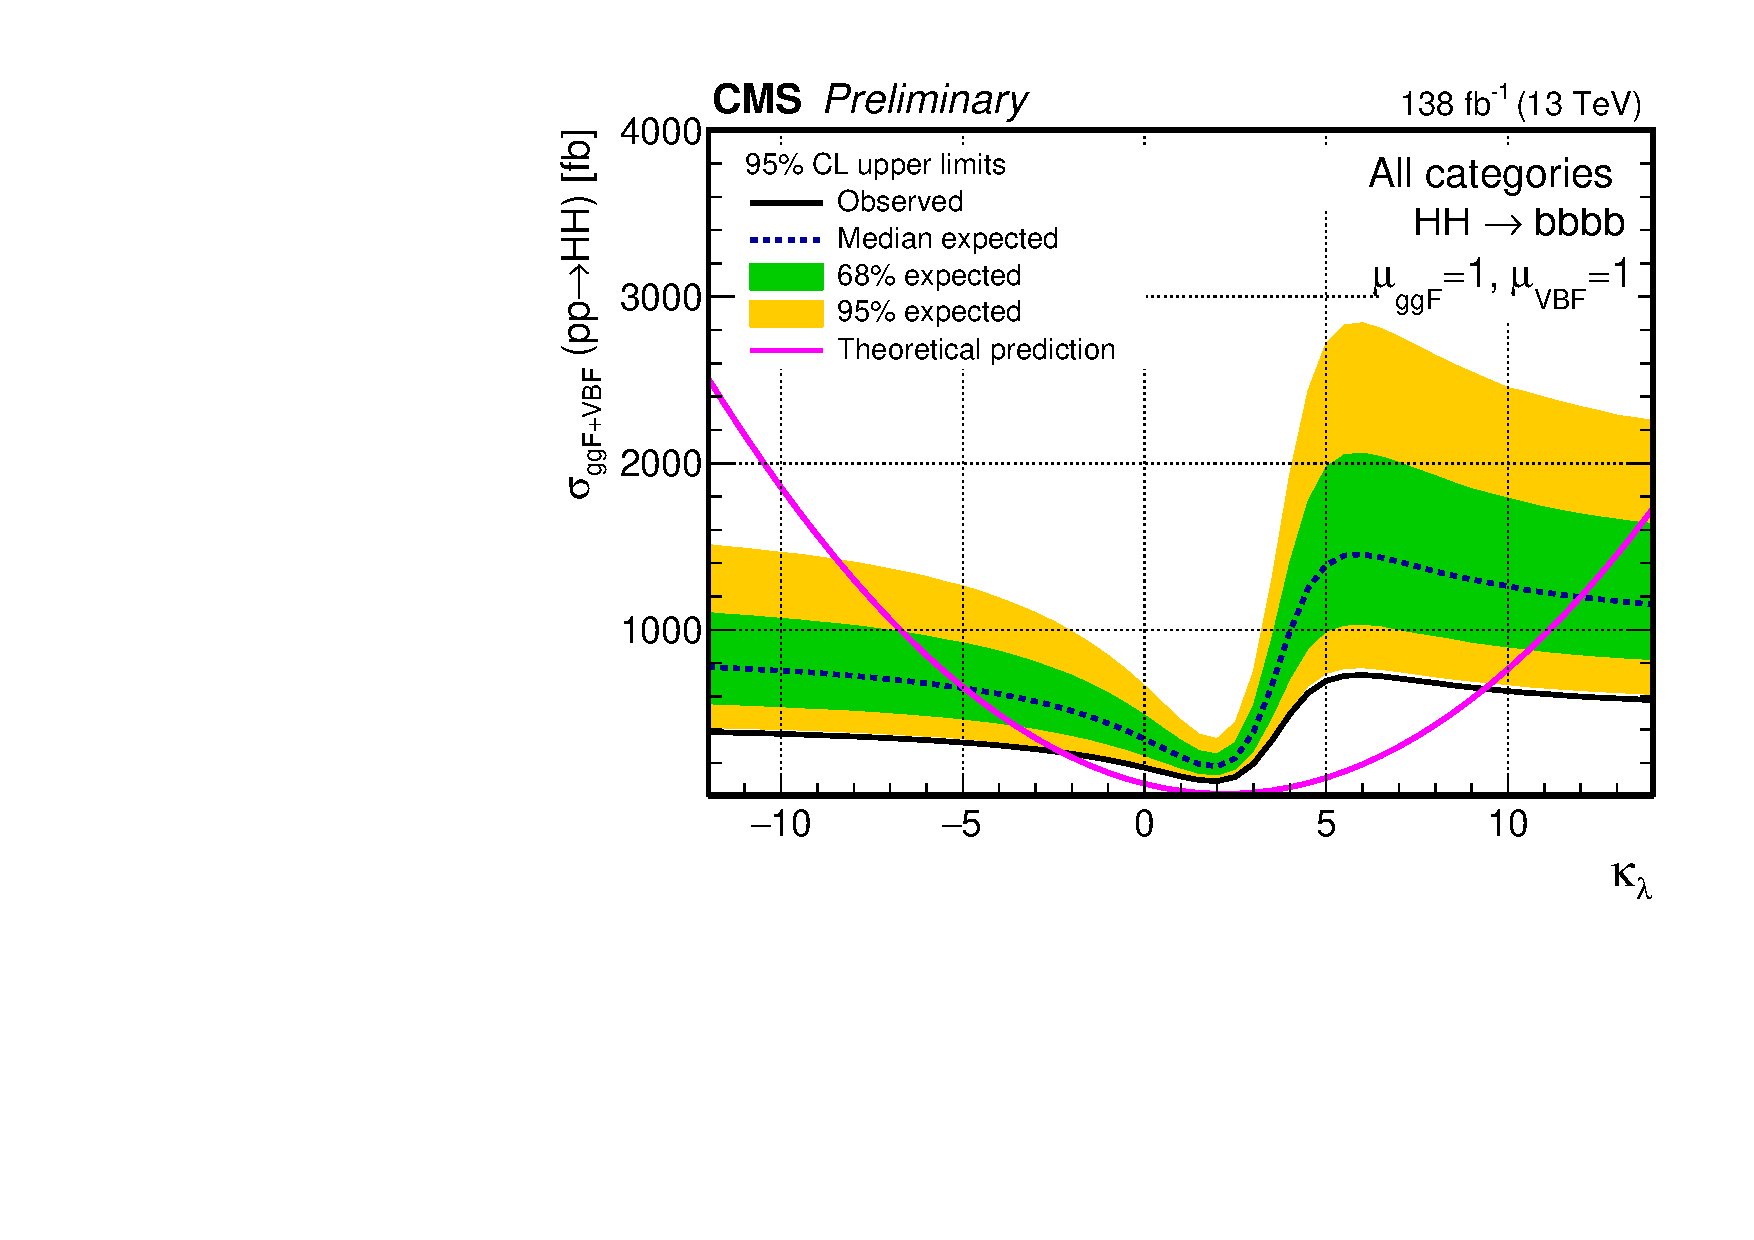
\includegraphics[width=0.50\linewidth]{Figures/Results/limits/CMS-PAS-HIG-20-005_Figure_002-a.pdf}}\hspace{\fill}}
\subfloat[]{{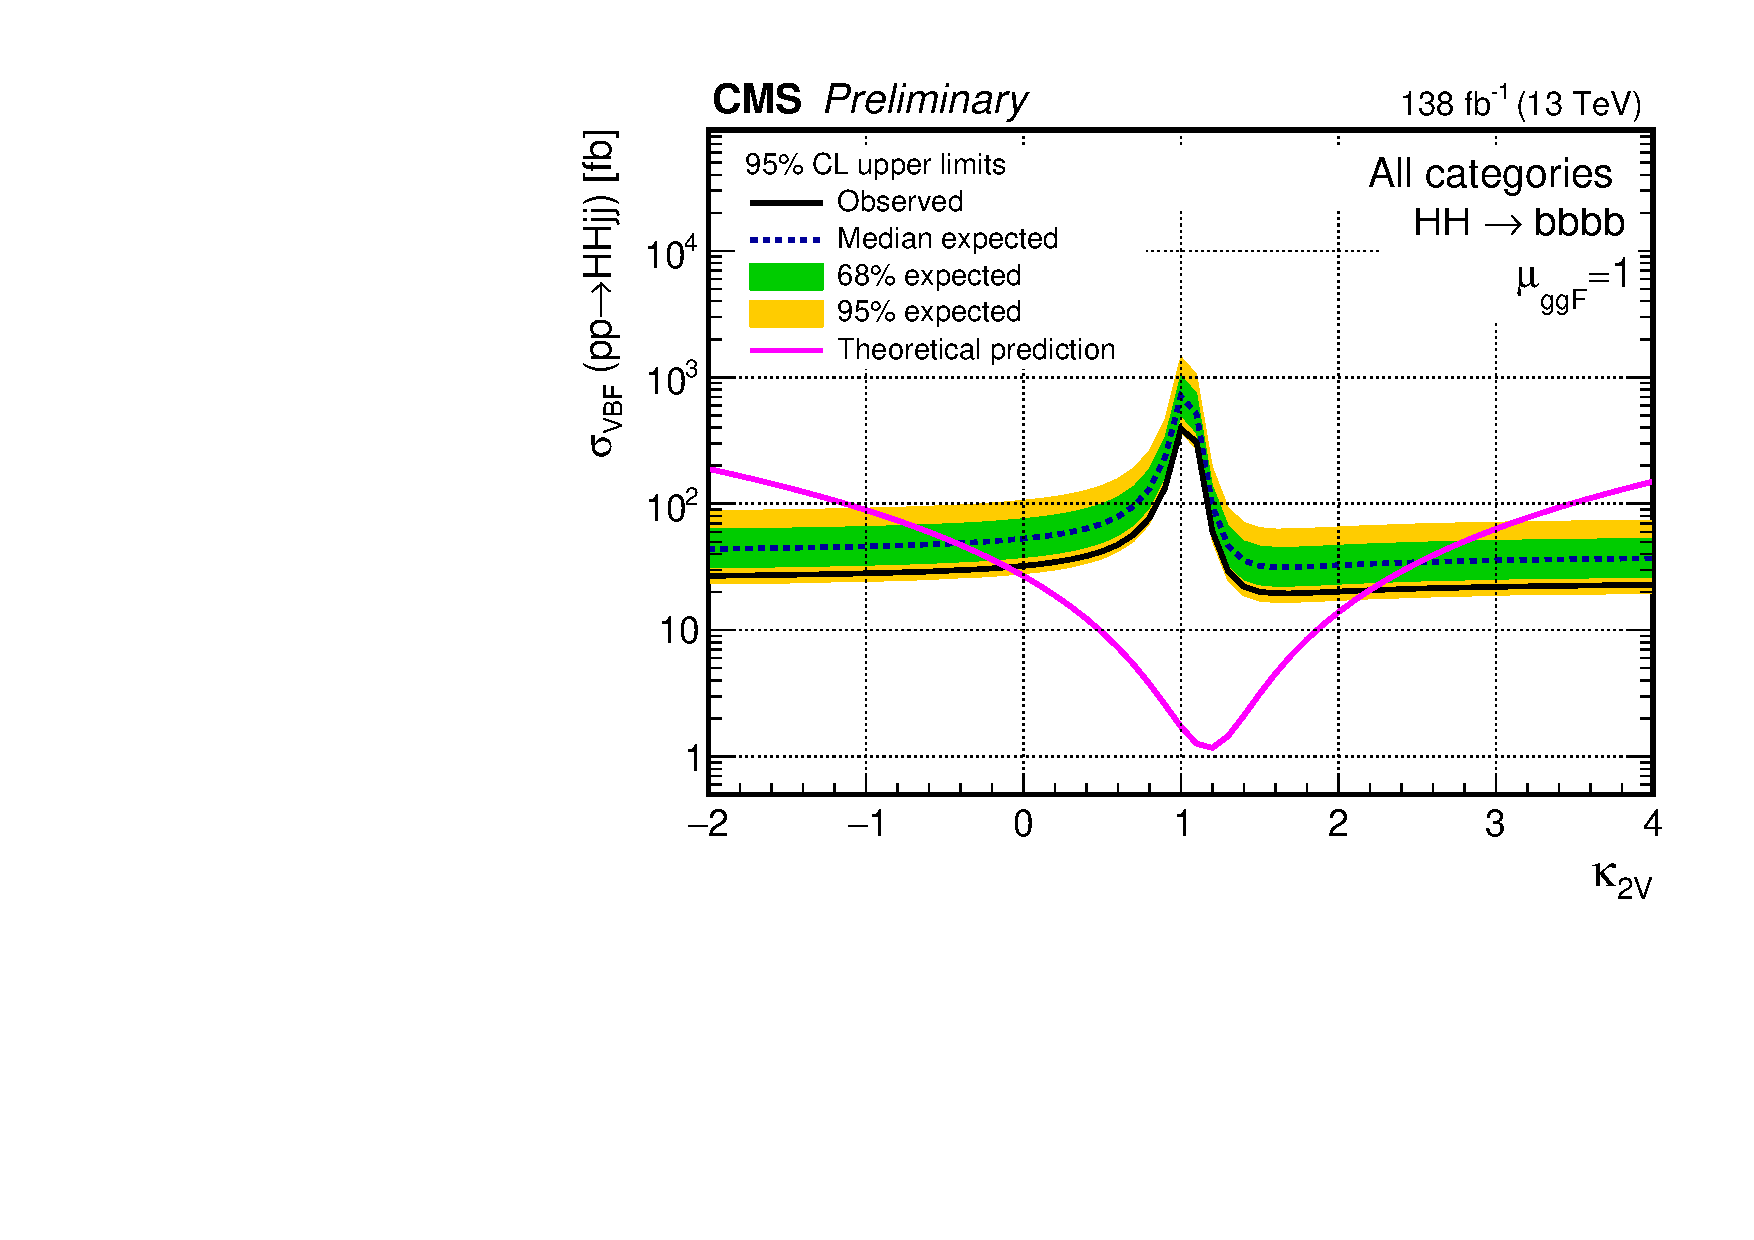
\includegraphics[width=0.50\linewidth]{Figures/Results/limits/CMS-PAS-HIG-20-005_Figure_002-b.pdf}}}
\caption[Observed and expected 95\% CL upper limits on Higgs boson pair cross section as a function of the coupling modifiers]{\label{fig:ULscans}
Observed and expected 95\% CL upper limits on Higgs boson pair cross section as a function of the coupling modifiers. A) $\kl$ and B) $\kvv$.
}
\end{figure*}

\begin{figure*}[!htb]
\centering
{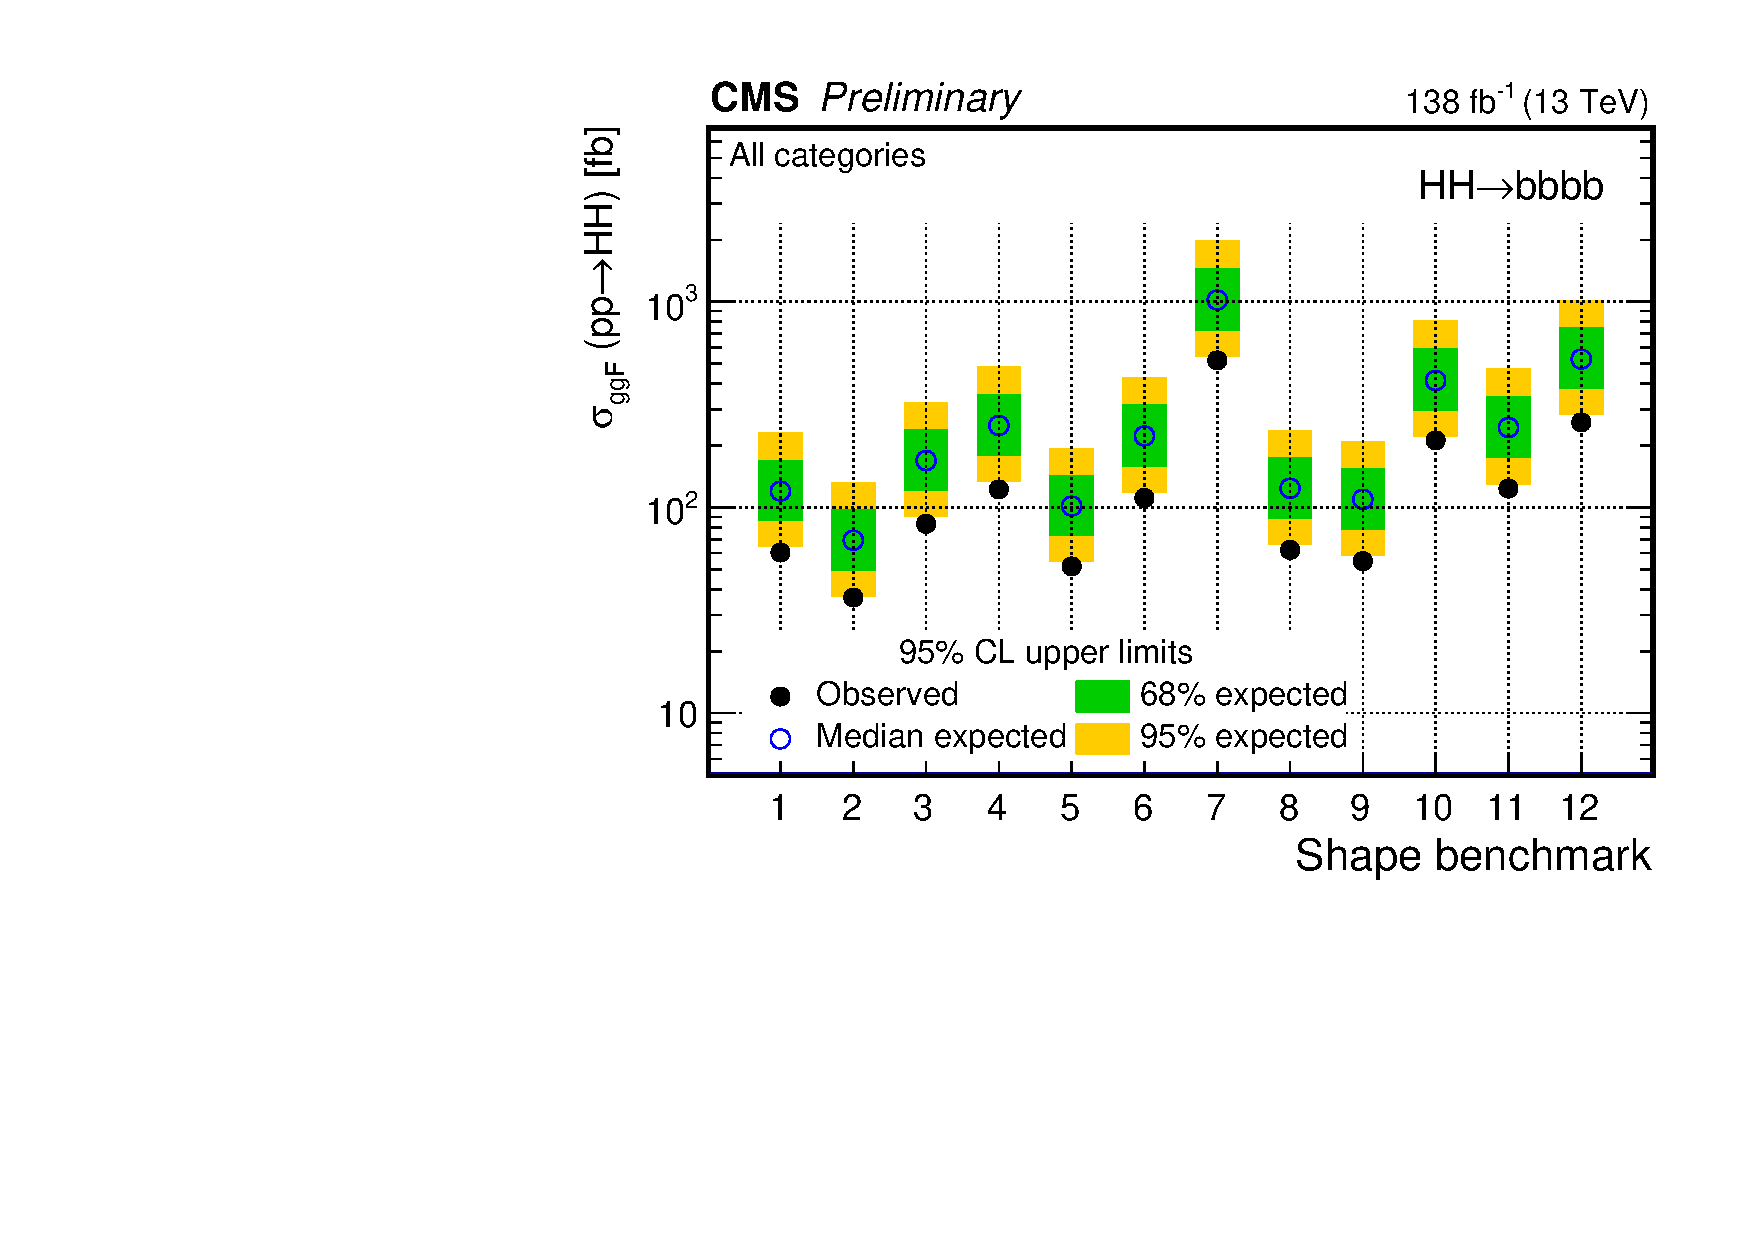
\includegraphics[width=0.50\linewidth]{Figures/Results/additional/CMS-PAS-HIG-20-005_Figure-aux_006.pdf}}
\caption[Observed and expected 95\% CL upper limits on the gluon fusion Higgs boson pair production cross section for the 12 benchmarks]{\label{fig:benchmarks}Observed and expected 95\% CL upper limits on the gluon fusion Higgs boson pair production cross section for the 12 benchmarks derived from the effective field theory parametrization.
}
\end{figure*}

\clearpage
\section{Likelihood Scans} \label{results:likelihoods}
Under the assumption that HH production exists according to the SM expectation, one can perform a measurement of the coupling modifiers through one dimensional or two-dimensional negative log-likelihood scans. The likelihood shape and minimum originates from an interplay between the cross section and the signal acceptance in the analysis categories. 

Figure~\ref{fig:likelihood_kl_c2V_1D} shows the one-dimensional negative log-likelihood scans as function of the $\kl$ (A) and $\kvv$ (B) coupling modifiers, where the coupling modifiers that are not shown in the figures are set to their SM values. The scans are evaluated with an Asimov dataset assuming the SM expected signal hypothesis (in light blue), and the observed data (black). In both cases, the observed likelihood is compatible with the SM hypothesis at 95\% CL.

\begin{figure*}[ht!]
\captionsetup[subfigure]{justification=centering}
\centering
\subfloat[]{{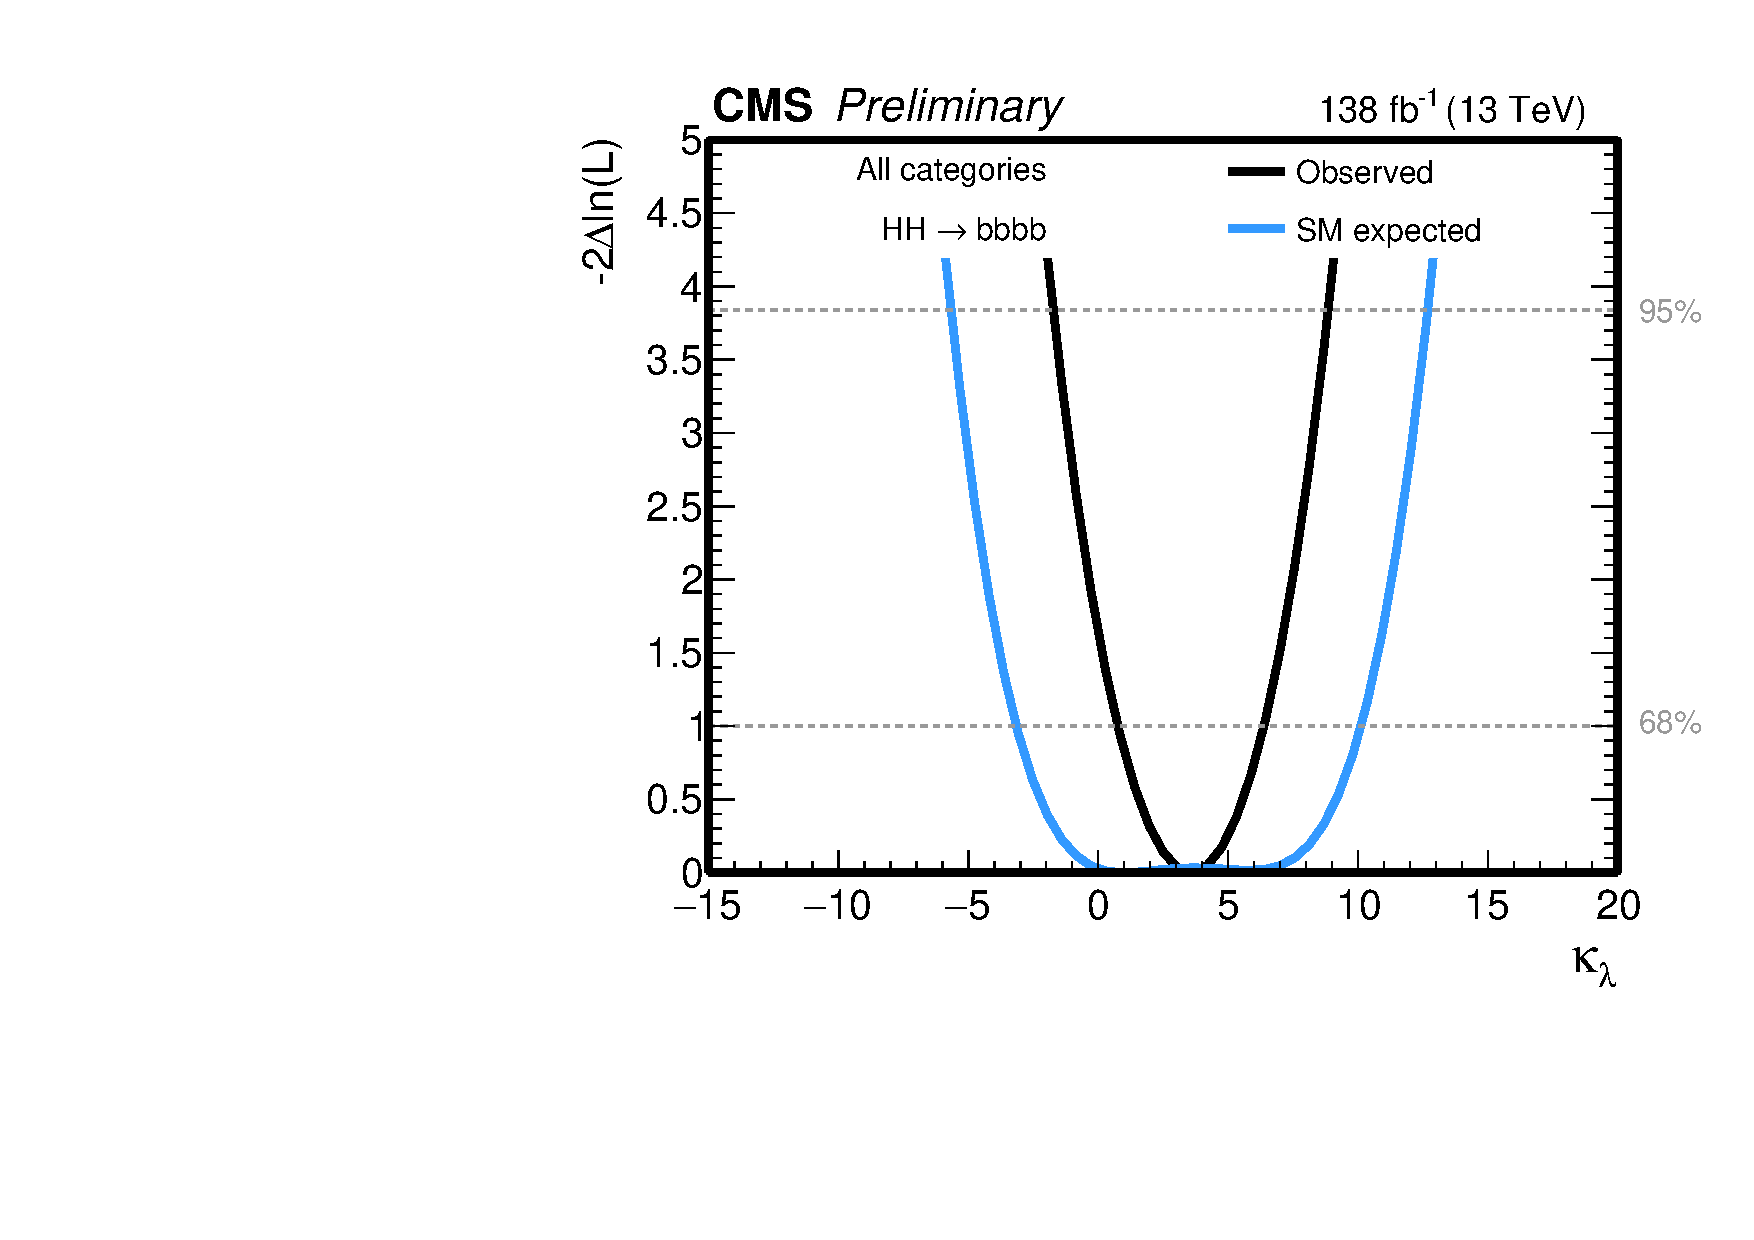
\includegraphics[width=0.50\linewidth] {Figures/Results/additional/CMS-PAS-HIG-20-005_Figure-aux_007-a.pdf}}\hspace{\fill}}
\subfloat[]{{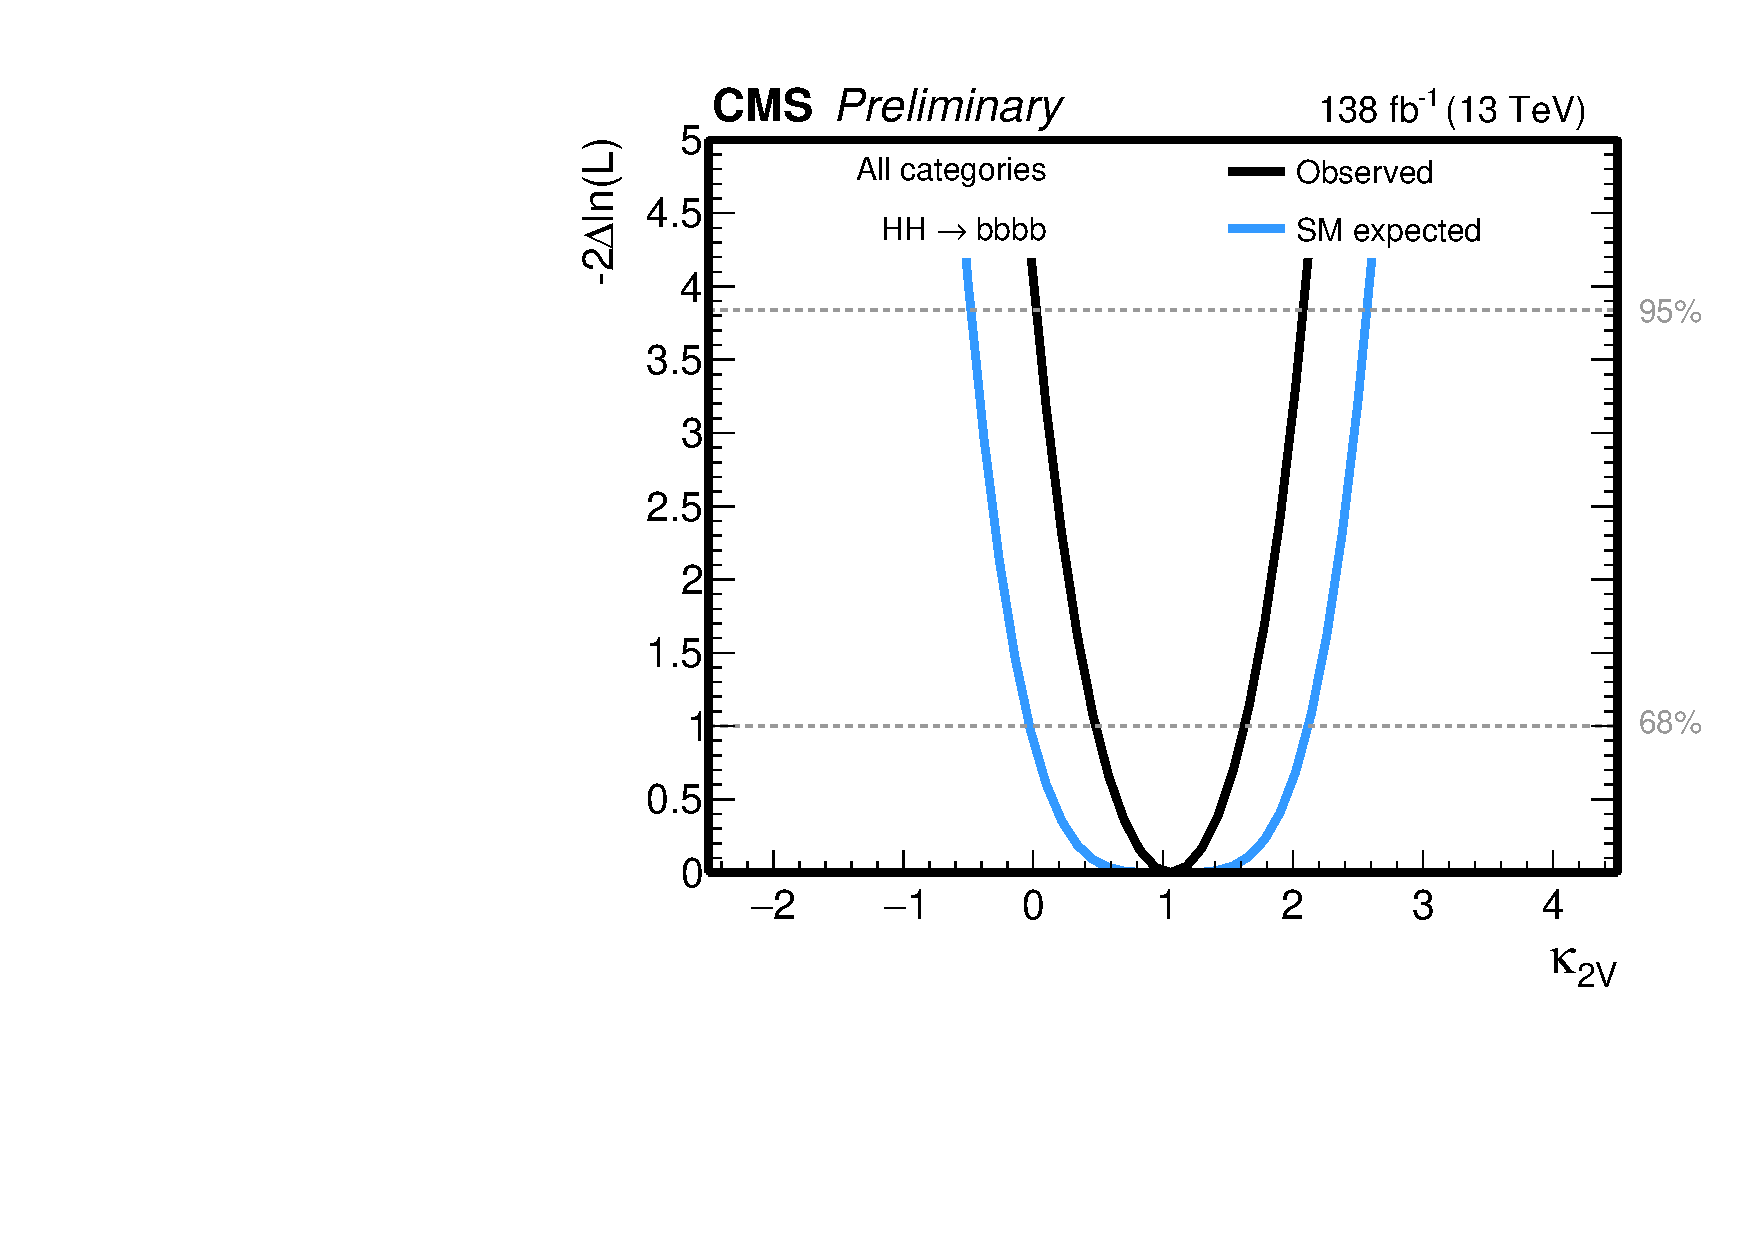
\includegraphics[width=0.50\linewidth] {Figures/Results/additional/CMS-PAS-HIG-20-005_Figure-aux_007-b.pdf}}}
\caption[Observed and expected negative log-likelihood scan as a function of the couplings]{\label{fig:likelihood_kl_c2V_1D}Observed and expected negative log-likelihood scan as a function of the couplings. A) $\kappa_{\lambda}$ and B) $\kappa_\text{2V}$ couplings.
}
\end{figure*}

Two-dimensional negative log-likelihood scans in the ($\kl$,$\kvv$) and ($\kvv$,$\kv$) planes are performed and illustrated in Figures~\ref{fig:likelihood_c2V_kl_2D} and ~\ref{fig:likelihood_c2V_kl_2D}, respectively.  The minimum or best-fit (black star) and the 68\% and 95\% CL contours are presented for both the Asimov dataset assuming the SM hypothesis and the observed data. The coupling modifiers not shown in the figures are set to the SM values. Both results in observed data are compatible with the SM expectation (circle) at 95\% CL.

\clearpage

\begin{figure*}[ht!]
\captionsetup[subfigure]{justification=centering}
\centering
\subfloat[]{{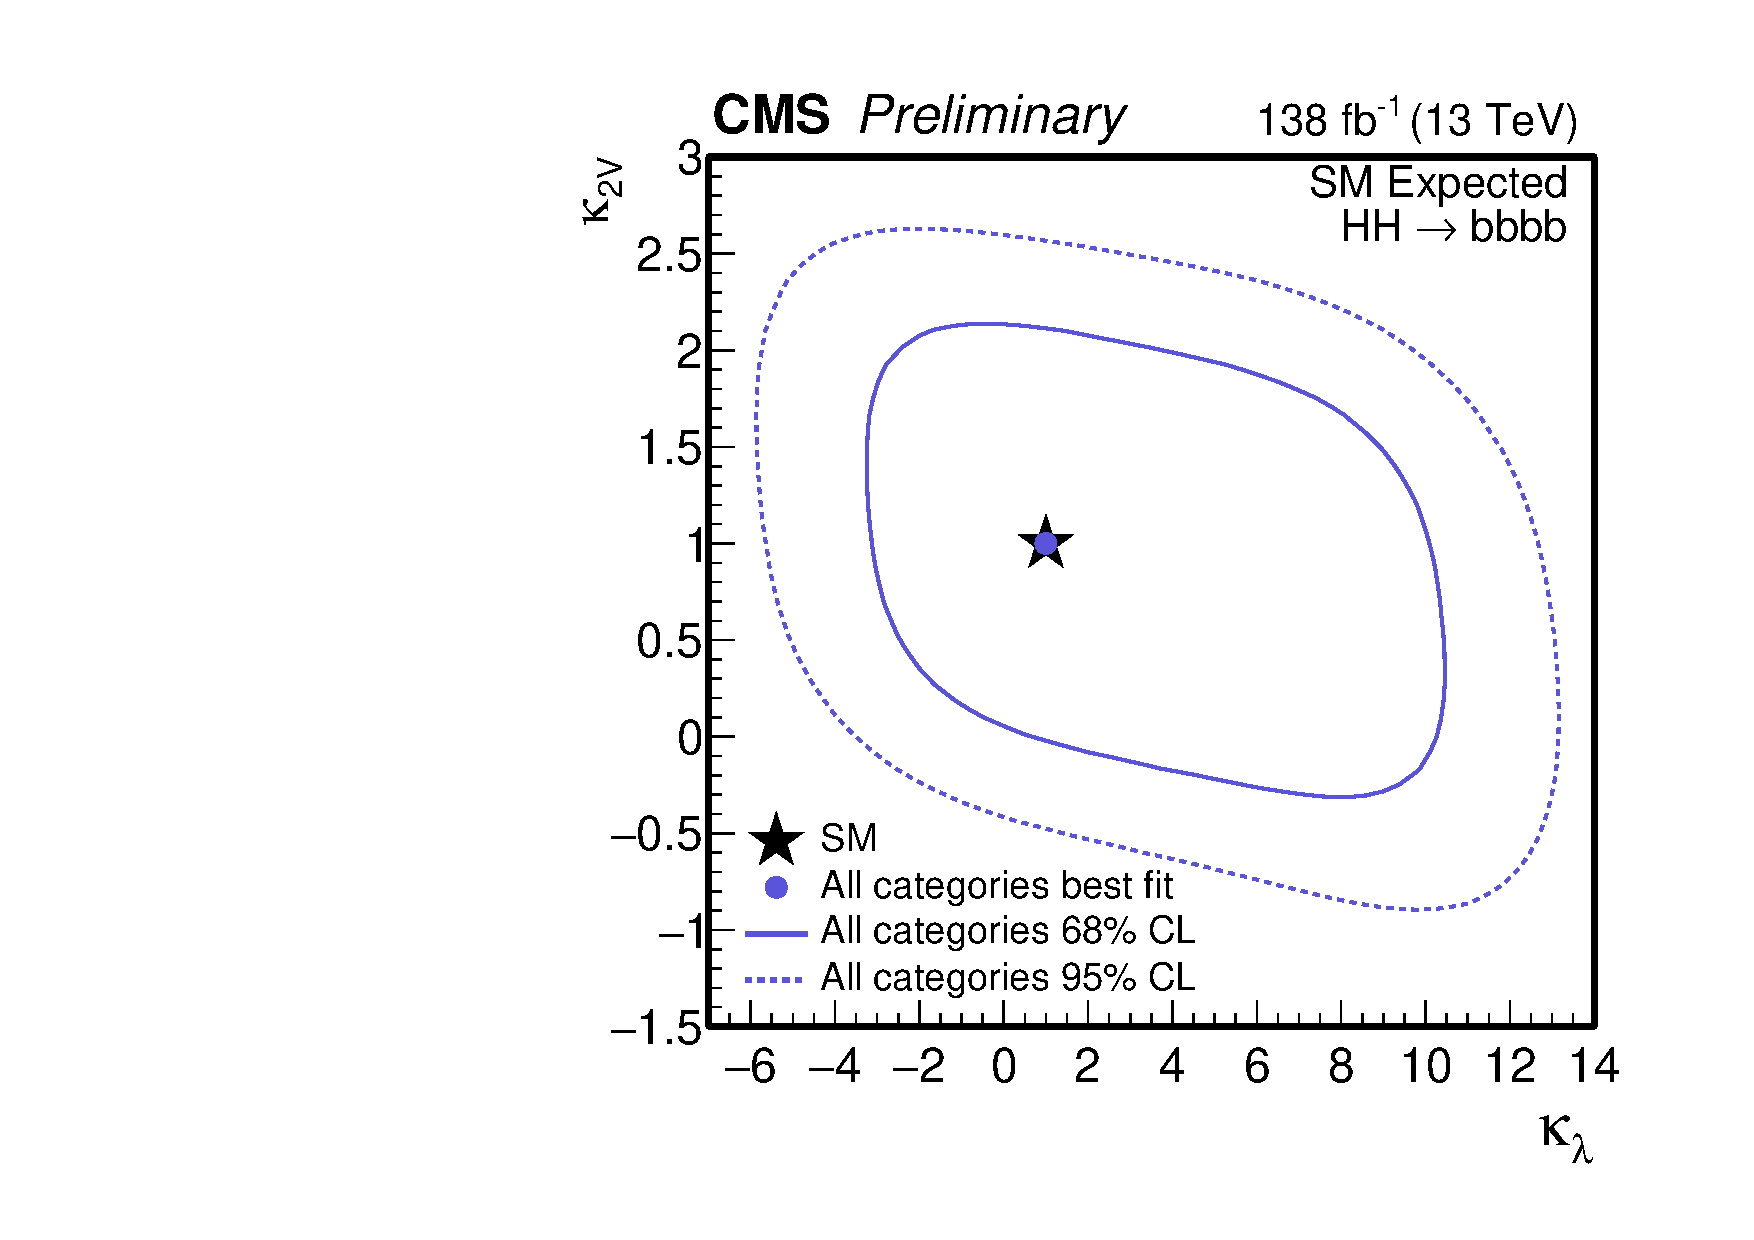
\includegraphics[width=0.48\linewidth] {Figures/Results/additional/CMS-PAS-HIG-20-005_Figure-aux_010-a.pdf}}}
\subfloat[]{{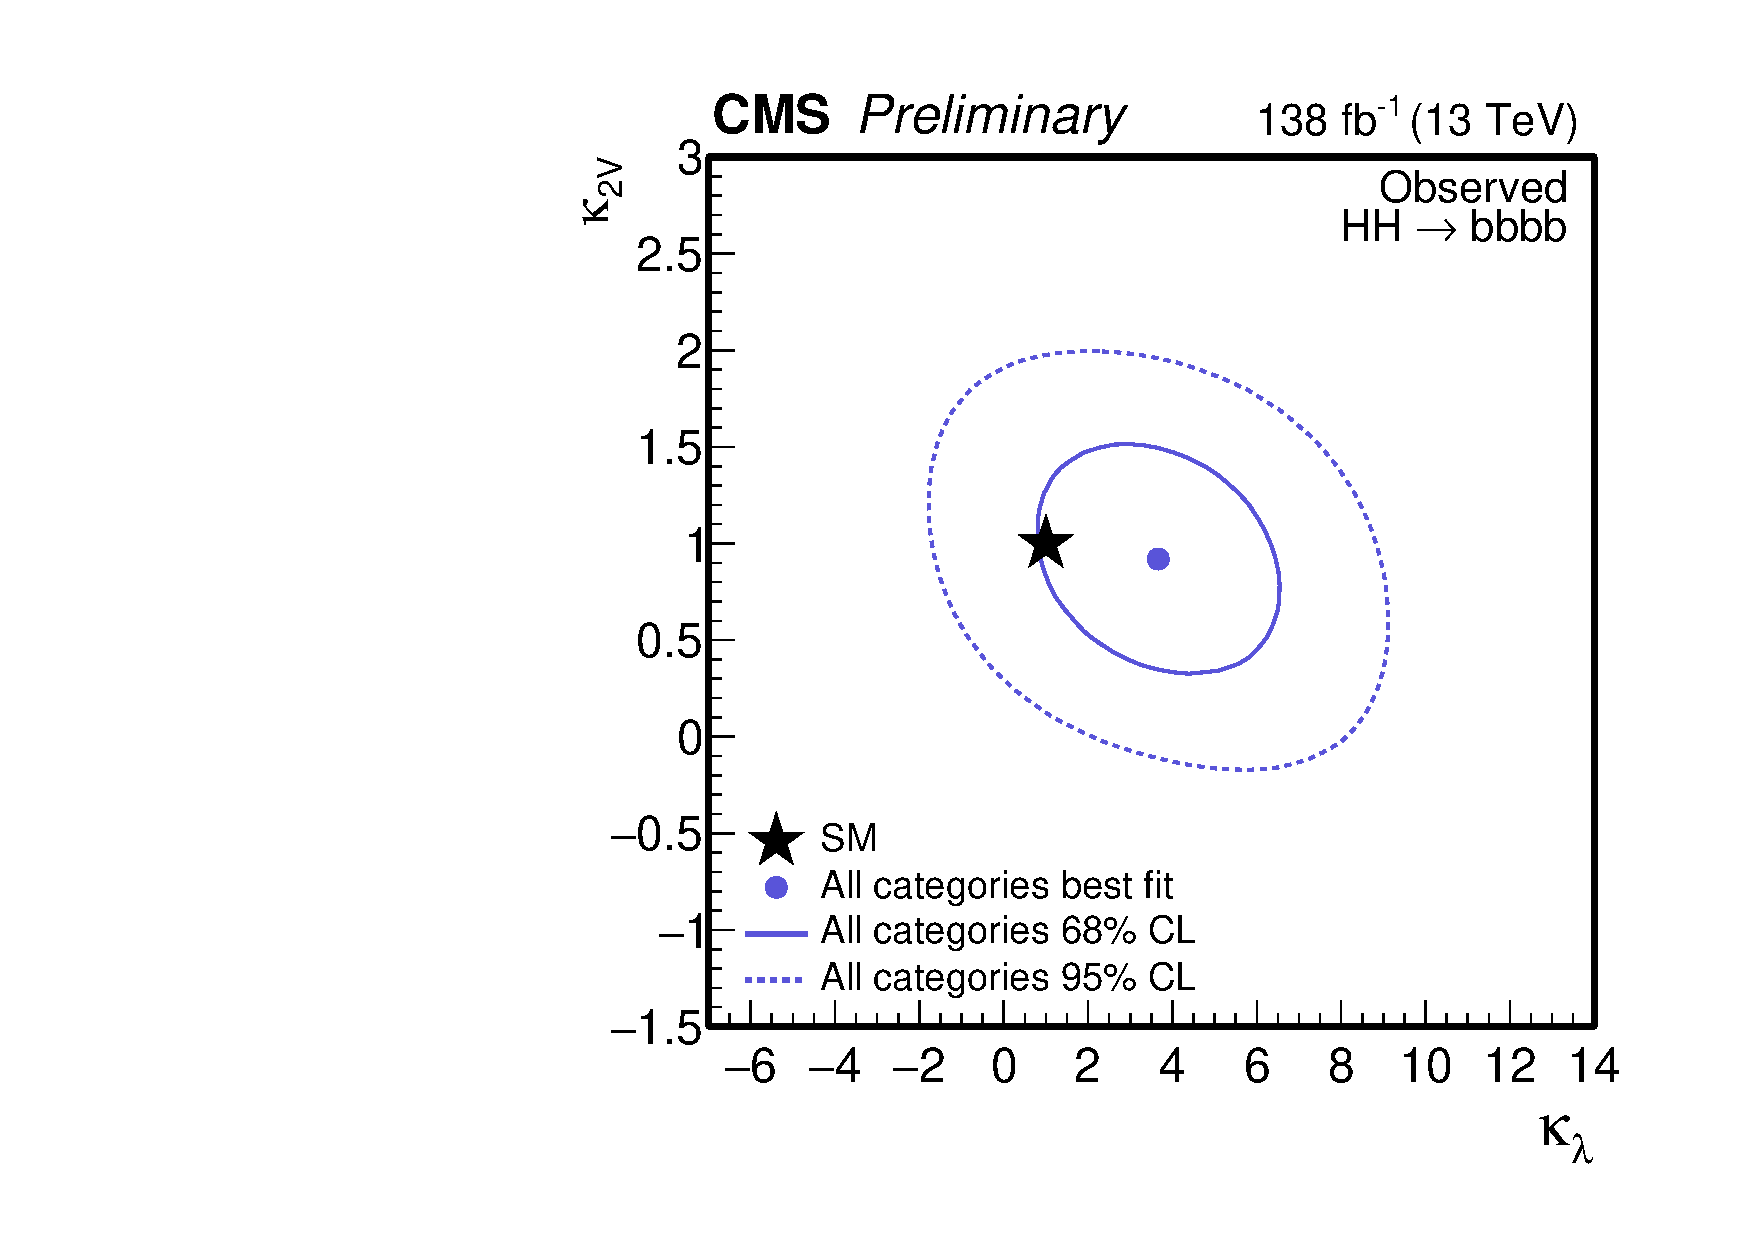
\includegraphics[width=0.48\linewidth] {Figures/Results/additional/CMS-PAS-HIG-20-005_Figure-aux_010-b.pdf}}}
\caption[Negative log-likelihood contours at 68\% and 95\% CL as a function of the ($\kl$,$\kvv$) couplings]{\label{fig:likelihood_c2V_kl_2D}Negative log-likelihood contours at 68\% and 95\% CL as a function of the ($\kl$,$\kvv$) couplings. A) SM hypothesis with Asimov dataset, and B) Observed data. The $\kt$ and $\kv$ couplings are set at the SM prediction.}
\end{figure*}

\begin{figure*}[ht!]
\captionsetup[subfigure]{justification=centering}
\centering
\subfloat[]{{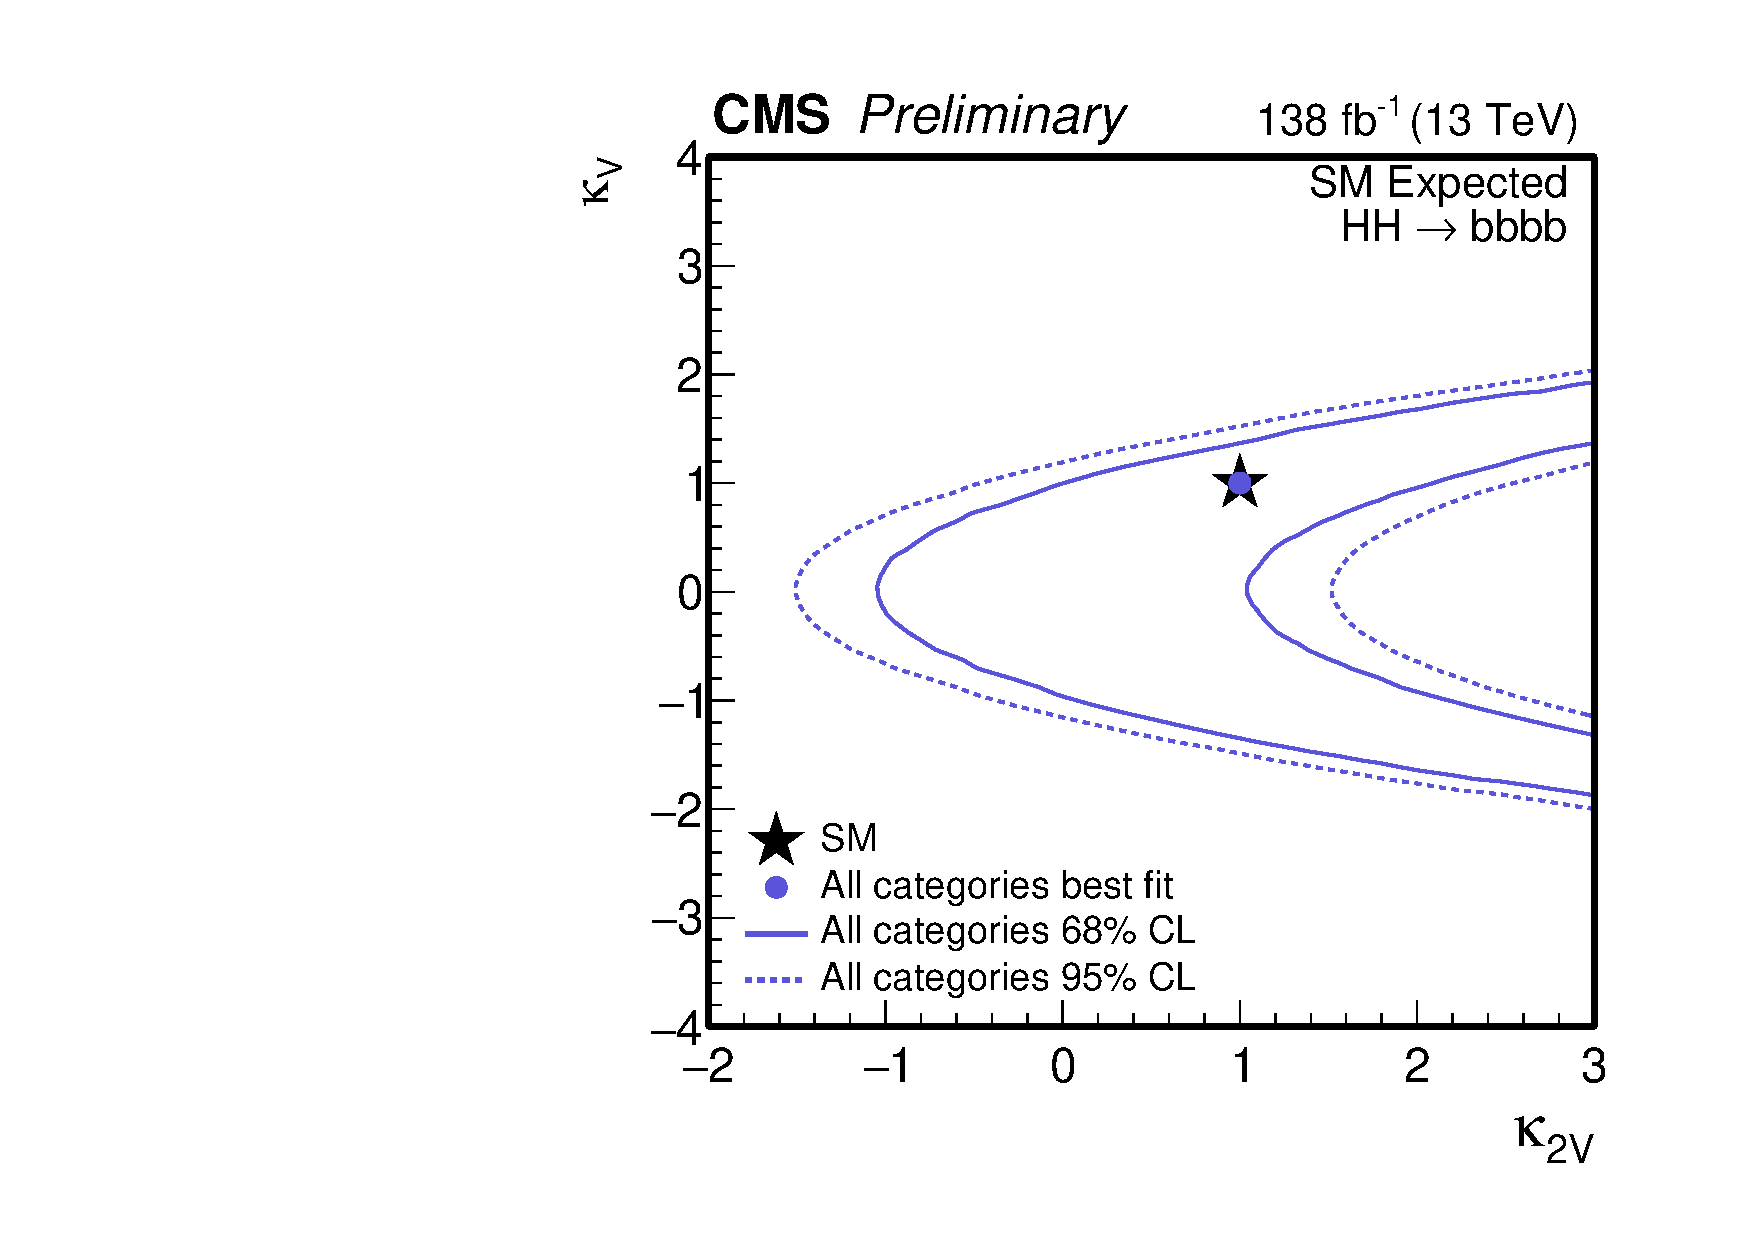
\includegraphics[width=0.48\linewidth] {Figures/Results/additional/CMS-PAS-HIG-20-005_Figure-aux_009-a.pdf}}}
\subfloat[]{{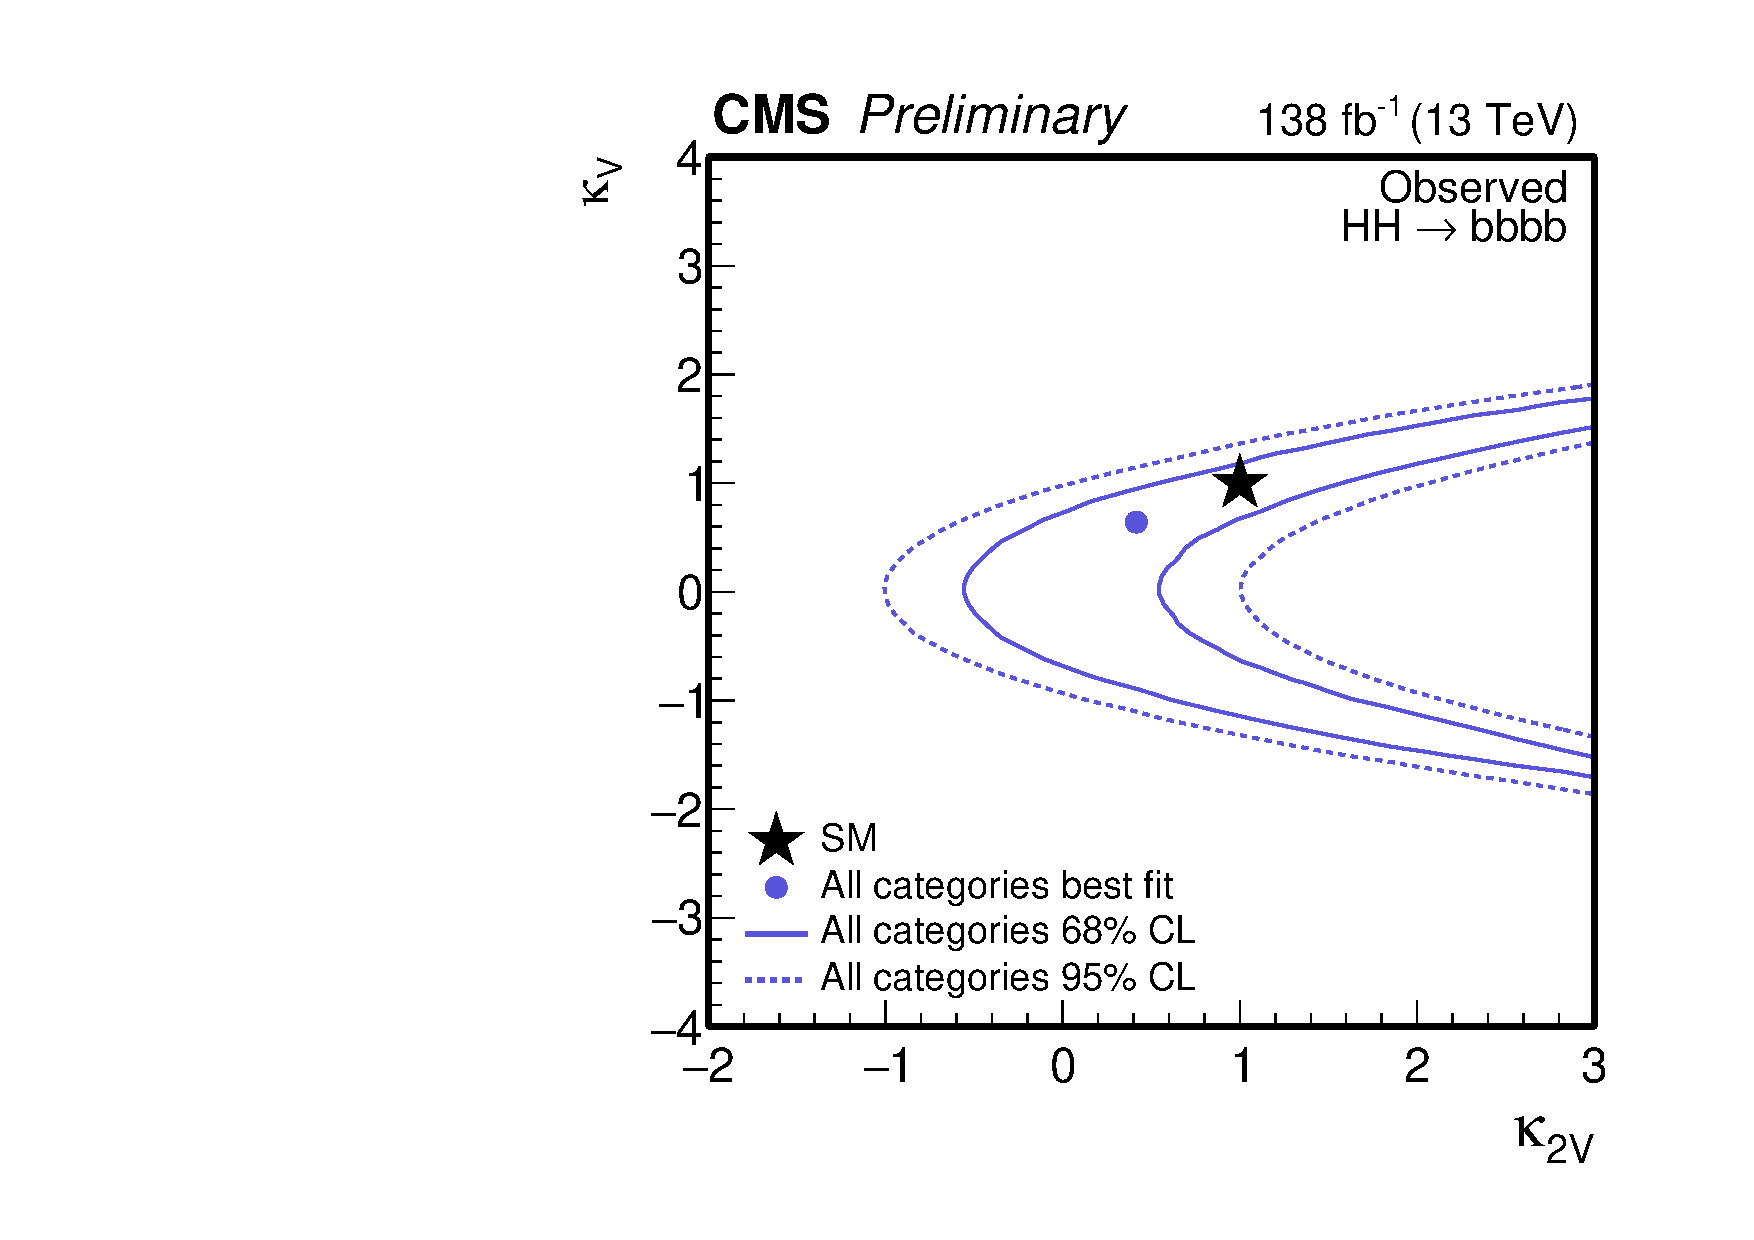
\includegraphics[width=0.48\linewidth] {Figures/Results/additional/CMS-PAS-HIG-20-005_Figure-aux_009-b.pdf}}}
\caption[Negative log-likelihood contours at 68\% and 95\% CL as a function of the ($\kvv$,$\kv$) couplings]{\label{fig:likelihood_c2V_cV_2D}Negative log-likelihood contours at 68\% and 95\% CL as a function of the ($\kvv$,$\kv$) couplings. A) SM hypothesis with Asimov dataset, and B) Observed data. The $\kl$ and $\kt$ couplings are set at the SM prediction.}
\end{figure*}